% SVN info for this file
\svnidlong
{$HeadURL$}
{$LastChangedDate$}
{$LastChangedRevision$}
{$LastChangedBy$}

\chapter{Gruppo fondamentale}
\labelChapter{gruppofonduta}

\begin{introduction}
	‘‘La Geometria algebrica sembra aver acquisito la reputazione di essere esoterica, esclusiva e molto astratta, con adepti che stanno segretamente complottando per impadronirsi di tutto il resto della Matematica. Da un certo punto di vista quest'ultimo punto è esatto.''
	\begin{flushright}
		\textsc{David Mumford,} assolutamente non un adepto della Geometria algebrica.
	\end{flushright}
\end{introduction}
\lettrine[findent=1pt, nindent=0pt]{N}{el} \autoref{chap:omotopia}, abbiamo studiato diverse proprietà legate all'\textit{omotopia}, mostrando alcuni esempi di spazi omotopicamente equivalenti. Tuttavia, non abbiamo ancora formalizzato un aspetto dell'intuizione iniziale: come contiamo i \textit{buchi} di una figura?\\
In questo capitolo proseguiamo la trattazione introducendo un \textit{oggetto algebrico} che associamo come invariante ad uno spazio topologico: il \textbf{gruppo fondamentale}. Definendo una versione dell'omotopia specifica dei cammini, utilizziamo questo gruppo formato dalle classi di equivalenza omotopica di \textit{cammini chiusi} per mostrare in termini rigorosi la presenza di buchi.\\
Inoltre, largo spazio sarà lasciato alla dimostrazione del primo gruppo fondamentale non banale, quello della \textit{circonferenza}.
\section{Omotopie fra cammini}
\begin{notation}{n}
Se non specificato differentemente, useremo $I$ per indicare l'intervallo $\unint$ con la topologia euclidea.
\end{notation}
\begin{definition}{}[Omotopia di cammini]
	Siano $\funct{}[\alpha,\beta]{I}{X}$ due cammini \textit{entrambi} da $a$ a $b$. Allora $\alpha,\ \beta$ sono \textbf{cammini omotopi}\index{cammino!omotopo} se esiste $\funct{}[F]{I \times I}{X}$ tale che
	\begin{align*}
			\begin{cases}
				F\left(t,0\right)=\alpha\left(t\right)\\
				F\left(t,1\right)=\beta\left(t\right)
			\end{cases}&
		\forall t\in I\ \text{ è omotopia tra } \alpha \text{ e }\beta;\\
	\end{align*}
	e
	\begin{align*}		
			\begin{cases}
			F\left(0,s\right)=a\\
			F\left(1,s\right)=b
		\end{cases}&
		\forall s\in I\ F\left(\cdot,s\right) \text{ è sempre un cammino tra } a \text{ e }b
	\end{align*}
	\begin{center}
		\includegraphics[trim=0cm 0cm 0cm 0cm,clip,scale=0.4]{images/pathhomotopy.pdf}
	\end{center}
$F$ è detta \textbf{omotopia di cammini}\index{omotopia!di cammini} o \textbf{omotopia a estremi fissi} \seeonlyindex{omotopia!a estremi fissi}{omotopia!di cammini}.
\end{definition}
\begin{definition}{}[Insieme dei cammini]
	Indichiamo con $\pathset{X}{a,b}$ l'\textbf{insieme dei cammini}\index{cammino!insieme dei cammini} in $X$ da $a$ a $b$.
\end{definition}
\begin{remark}{n}
	L'omotopia di cammini è una relazione di equivalenza su $\pathset{X}{a,b}$.
\end{remark}
\begin{proof}{n}~{}
		\begin{itemize}
		\item \textit{Riflessività}: presa $F\left(t,s\right)\coloneqq\alpha\left(t\right)$, essa è ben definita, continua e
		\begin{equation*}
			F\left(t,0\right)=\alpha\left(t\right),\ F\left(t,1\right)=\alpha\left(t\right),\ F\left(0,s\right)=\alpha\left(0\right)=a,\ F\left(1,s\right)=\alpha\left(1\right)=b,
		\end{equation*}
	cioè è omotopia di cammini tra $\alpha$ e $\alpha$ e quindi $\alpha\sim \alpha$.
		\item \textit{Simmetria}: da $\alpha\sim \beta$ sappiamo che esiste $F$ omotopia di cammini per cui
		\begin{equation*}
			\begin{cases}
				F\left(t,0\right)=\alpha\left(t\right)\\
				F\left(t,1\right)=\beta\left(t\right)
			\end{cases}
		\end{equation*}
		Per avere $\beta\sim \alpha$, poniamo $\widetilde{F}\left(t,s\right)\coloneqq F\left(t,1-s\right)$: essa è ben definita, continua e
		\begin{gather*}
			\widetilde{F}\left(t,0\right)=F\left(t,1\right)=\beta\left(t\right),\ \widetilde{F}\left(t,1\right)=F\left(t,0\right)=\alpha\left(t\right)\\
			\widetilde{F}\left(0,s\right)=F\left(0,s\right)=a,\ \widetilde{F}\left(1,s\right)=F\left(1,s\right)=b
		\end{gather*}
		cioè è omotopia di cammini tra $\beta$ e $\alpha$ e quindi $\beta\sim \alpha$.
		\item \textit{Transitività}: da $\alpha\sim \beta$ abbiamo
	\begin{equation*}
			\begin{array}{ll}
			\begin{cases}
				F\left(t,0\right)=\alpha\left(t\right)\\
				F\left(t,1\right)=\beta\left(t\right)
			\end{cases}&
		\begin{cases}
				F\left(0,s\right)=a\\
				F\left(1,s\right)=b
		\end{cases}
			\end{array}
	\end{equation*}
mentre da $\beta\sim \gamma$
	\begin{equation*}
	\begin{array}{ll}
		\begin{cases}
			G\left(t,0\right)=\beta\left(t\right)\\
			G\left(t,1\right)=\gamma\left(t\right)
		\end{cases}&
	\begin{cases}
			G\left(0,s\right)=a\\
			G\left(1,s\right)=b
	\end{cases}
	\end{array}
\end{equation*}
Definita allora la seguente funzione
\begin{equation*}
	H\left(t,s\right)\coloneqq\begin{cases}
			F\left(t,2s\right)&\text{se }s\in\left[0,\ \frac{1}{2}\right]\\
			G\left(t,2s-1\right)&\text{se }s\in\left[\frac{1}{2},\ 1\right]
	\end{cases}
\end{equation*}
Essa è ben definita, continua per il lemma di incollamento e tale per cui
\begin{gather*}
	H\left(t,0\right)=F\left(t,0\right)=\alpha\left(t\right),\ H\left(t,1\right)=G\left(t,1\right)=\gamma\left(t\right)\\
	H\left(0,s\right)=a,\ H\left(1,s\right)=b
\end{gather*}
		cioè è omotopia di cammini tra $\alpha$ e $\gamma$ e dunque $\alpha\sim\gamma$.\qedhere
	\end{itemize}
\end{proof}
\begin{remember}{n}
Abbiamo già definito due ‘‘operazioni'' fra insiemi di cammini, senza averle necessariamente formalizzate:
\begin{itemize}
\item \textit{Prodotto di cammini}:
\begin{equation*}
	\funct{}[\ast]{\pathset{X}{a,b}\times\pathset{X}{b,c}}{\pathset{X}{a,c}}[\left(\alpha,\ \beta\right)][\alpha\ast\beta]
\end{equation*}
\item \textit{Inversione di cammini}:
\begin{equation*}
	\funct{}[\overline{\cdot}]{\pathset{X}{a,b}}{\pathset{X}{b,a}}[\alpha][\overline{\alpha}]
\end{equation*}
\end{itemize}
\end{remember}
\begin{remark}{n}
Si ha $\overline{\overline{\alpha}}=\alpha$. Infatti, essendo $\overline{\alpha}\left(t\right)=\alpha\left(1-t\right)$, si ha
\begin{equation*}
	\implies\overline{\overline{\alpha}}\left(t\right)=\overline{\alpha}\left(1-t\right)=\alpha\left(t\right)
\end{equation*}
\end{remark}
\begin{lemma}{}[Composizioni di omotopie di cammini; Kosniowski, 14.2]\label{compoomotopecammini}
Dati $\alpha,\ \alpha'\in\pathset{X}{a,b}$ e $\beta,\ \beta '\in\pathset{X}{b,c}$, in termini di omotopie di cammini:
	\begin{equation*}
		\alpha\sim \alpha'\text{ e }\beta\sim \beta'\implies \alpha\ast\beta\sim\alpha'\ast\beta'
	\end{equation*}
\end{lemma}
\begin{proof}{n}
	Esistono $\funct{}[F,G]{I\times I}{X}$ tali che
	\begin{gather*}
		\begin{cases}
			F\left(t,0\right)=\alpha\left(t\right)\\
			F\left(t,1\right)=\alpha'\left(t\right)
		\end{cases}
		\qquad
		\begin{cases}
			F\left(0,s\right)=a\\
			F\left(1,s\right)=b
		\end{cases}
	,\forall t,\ s\in I\\
	\begin{cases}
		G\left(t,0\right)=\beta\left(t\right)\\
		G\left(t,1\right)=\beta'\left(t\right)
	\end{cases}
	\qquad
	\begin{cases}
		G\left(0,s\right)=b\\
		G\left(1,s\right)=c
	\end{cases},\forall t,\ s\in I
	\end{gather*}
Consideriamo $\funct{}[H]{I\times I}{X}$ data da
\begin{equation*}
	H\left(t,s\right)\coloneqq
	\begin{cases}
			F\left(2t,s\right) & \text{se }0\leq t\leq \frac{1}{2}\\
			G\left(2t-1,s\right) & \text{se }\frac{1}{2}\leq t\leq 1
	\end{cases}
\end{equation*}
\begin{itemize}
	\item $H$ è ben definita per $t=\frac{1}{2}$.
	\item $H$ è continua per il lemma di incollamento, essendo definito sui chiusi $\left[0,\ \frac{1}{2}\right]\times I$ e $\left[\frac{1}{2},\ 1\right]\times I$ è continua su di essi.
	\item Per ogni $t$ è omotopia in quanto
	\begin{equation*}
		\begin{cases}
			H\left(t,0\right)=\left(\alpha\ast\beta\right)\left(t\right)\\
			H\left(t,1\right)=\left(\alpha'\ast\beta'\right)\left(t\right)
		\end{cases}
	\end{equation*}
	\item Per ogni $s\in I$ ha estremi fissi:
	\begin{equation*}
		\begin{cases}
			H\left(0,s\right)=F\left(0,s\right)=a\\
			H\left(1,s\right)=G\left(1,s\right)=c
		\end{cases}
	\end{equation*}
\end{itemize}
$F$ è l'omotopia a estremi fissi cercata.\qedhere
\end{proof}
\begin{lemma}{}[Cambiamento di parametri; Manetti, 11.3]\label{cambiamentodiparametri}
	Sia $\funct{}[\alpha]{I}{X}$ un cammino e $\funct{}[\varphi]{I}{I}$ una funzione continua tale che $\varphi\left(0\right)=0$ e $\varphi\left(1\right)=1$. Allora $\alpha\circ \varphi\sim\alpha$.
\end{lemma}
\begin{proof}{n}
	Sia $\funct{}[F]{I\times I}{X}$ data da $F\left(t,s\right)\coloneqq\alpha\left(s\varphi\left(t\right)+\left(1-s\right)t\right)$.
	\begin{itemize}
		\item $s\varphi\left(t\right)+\left(1-s\right)t$ è una combinazione lineare che è contenuta in $I\subseteq \R\ \forall t,\ s\in I$ per convessità dell'intervallo $I$, da cui segue che $F$ è ben definita.
		\item $F$ continua perché composizione di funzioni continue.
		\item Per ogni $t\in I$ è omotopia in quanto
		\begin{equation*}
			\begin{cases}
				F\left(t,0\right)=\alpha\left(t\right)\\
				F\left(t,1\right)=\alpha\left(\varphi\left(t\right)\right)
			\end{cases}
		\end{equation*}
		\item Per ogni $s\in I$ ha estremi fissi:
		\begin{equation*}
			\begin{cases}
				F\left(0,s\right)=\alpha\left(0\right)\\
				F\left(1,s\right)=\alpha\left(s+1-s\right)=\alpha\left(1\right)
			\end{cases}
		\end{equation*}
	\end{itemize}
$H$ è l'omotopia a estremi fissi cercata tra $\alpha$ e $\alpha\circ\varphi$.
\end{proof}
\begin{definition}{}[Cammino costante]
	Il \textbf{cammino costante} $C_a$\index{cammino!costante} nel punto $a$ è un cammino che non si sposta mai da esso, cioè è descritto dalla funzione costante nel punto
	\begin{equation*}
		\funct{}[C_a]{I}{X}[t][a]
	\end{equation*}
\end{definition}
\begin{property}{}[Proprietà dell'omotopia di cammini; Manetti, 11.4 e 11.6]\label{propcammini}
Sia $X$ spazio topologico e si considerino i cammini
	\begin{equation*}
	\alpha\in\pathset{X}{a,b}\quad\beta\in\pathset{X}{b,c}\quad\gamma\in\pathset{X}{c,d}
	\end{equation*}
Valgono le seguenti proprietà:
\begin{enumerate}
	\item \textit{Associatività}: $\left(\alpha\ast\beta\right)\ast \gamma \sim \alpha\ast\left(\beta\ast\gamma\right)$.
	\item \textit{Rapporto coi cammini costanti}: $C_a\ast \alpha \sim \alpha \sim \alpha \ast C_b$.
	\item \textit{Inverso}: $\alpha\ast\overline{\alpha}\sim C_a$ e $\overline{\alpha}\ast\alpha\sim C_a$.
\end{enumerate}
\end{property}
\begin{proof}{n}~{}
\begin{enumerate}[label=\Roman*]
	\item Scriviamo i due cammini:
	\begin{gather*}
\left(\left(\alpha\ast\beta\right)\ast\gamma\right)\left(t\right)=\begin{cases}
	\begin{array}{ll}
		\alpha\left(4t\right)&t\in\left[0,\ \frac{1}{4}\right]\\
		\beta\left(4t-1\right)&t\in\left[\frac{1}{4},\ \frac{1}{2}\right]\\
		\gamma\left(2t-1\right)&t\in\left[\frac{1}{2},\ 1\right]
	\end{array}
\end{cases}\\
\left(\left(\alpha\ast\left(\beta\ast\gamma\right)\right)\right)\left(t\right)=\begin{cases}
\begin{array}{ll}
	\alpha\left(2t\right)&t\in\left[0,\ \frac{1}{2}\right]\\
	\beta\left(4t-2\right)&t\in\left[\frac{1}{2},\ \frac{3}{4}\right]\\
	\gamma\left(4t-3\right)&t\in\left[\frac{3}{4},\ 1\right]
\end{array}
\end{cases}
	\end{gather*}
I due cammini differiscono per una \textit{riparametrizzazione} $\funct{}[\oldphi]{I}{I}$ di $\alpha\ast\left(\beta\ast\gamma\right)$ definita in questo modo:
\begin{gather*}
	\begin{cases}
		\begin{array}{l}
			2s=4t\\
			4s-2=4t-1\\
			4s-3=2t-1
		\end{array}
\implies
\begin{cases}
\begin{array}{ll}
	s=2t&t\in\left[0,\ \frac{1}{4}\right]\\
	s=t+\frac{1}{4}&t\in\left[\frac{1}{4},\ \frac{1}{2}\right]\\
	s=\frac{t}{2}+\frac{1}{2}&t\in\left[\frac{1}{2},\ 1\right]
\end{array}
		\end{cases}
	\end{cases}\\
\oldphi\left(t\right)=	\begin{cases}
\begin{array}{ll}
	2t&t\in\left[0,\ \frac{1}{4}\right]\\
	t+\frac{1}{4}&t\in\left[\frac{1}{4},\ \frac{1}{2}\right]\\
	\frac{t}{2}+\frac{1}{2}&t\in\left[\frac{1}{2},\ 1\right]
\end{array}
		\end{cases}
\end{gather*}
\begin{itemize}
	\item $\oldphi$ è ben definita e continua per lemma di incollamento.
	\item $\oldphi\left(0\right)=0$ e $\oldphi\left(1\right)=1$.
	\item $\left(\left(\alpha\ast\left(\beta\ast\gamma\right)\right)\right)\left(\oldphi\left(t\right)\right)=\left(\left(\alpha\ast\beta\right)\ast\gamma\right)\left(t\right)$.
\end{itemize}
Per il lemma del cambiamento di parametro i due cammini sono omotopi.
\item Scriviamo i due cammini:
\begin{gather*}
	\left(C_a\ast \alpha\right)\left(t\right)=\begin{cases}
		\begin{array}{ll}
			a&t\in\left[0,\ \frac{1}{2}\right]\\
			\alpha\left(2t-1\right)&t\in\left[\frac{1}{2},\ 1\right]
		\end{array}
	\end{cases}\\
	\left(\alpha\ast C_b\right)\left(t\right)=\begin{cases}
		\begin{array}{ll}
			\alpha\left(2t\right)&t\in\left[0,\ \frac{1}{2}\right]\\
			b&t\in\left[\frac{1}{2},\ 1\right]
		\end{array}
	\end{cases}
\end{gather*}
I due cammini differiscono per delle \textit{riparametrizzazioni} di $\alpha$, che denotiamo con $\funct{}[\oldphi]{I}{I}$ e $\funct{}[\psi]{I}{I}$, definite così:
\begin{equation*}
	\oldphi\left(t\right)=
	\begin{cases}
		\begin{array}{ll}
			0&t\in\left[0,\ \frac{1}{2}\right]\\
			2t-1&t\in\left[\frac{1}{2},\ 1\right]
		\end{array}
	\end{cases}
\qquad	\psi\left(t\right)=
\begin{cases}
	\begin{array}{ll}
		2t&t\in\left[0,\ \frac{1}{2}\right]\\
		1&t\in\left[\frac{1}{2},\ 1\right]
	\end{array}
\end{cases}
\end{equation*}
\begin{itemize}
	\item $\oldphi$ e $\psi$ son ben definite e continue per lemma di incollamento.
	\item $\oldphi\left(0\right)=0,\ \psi\left(0\right)=0$ e $\oldphi\left(1\right)=1,\psi\left(1\right)=1 $.
	\item $\left(C_a\ast \alpha\right)\left(t\right)=\alpha\left(\oldphi\left(t\right)\right)$ e $\left(\alpha\ast C_b\right)\left(t\right)=\alpha\left(\psi\left(t\right)\right)$.
\end{itemize}
Per il lemma del cambiamento di parametro i due cammini sono entrambi omotopi a $\alpha$, si hanno quindi le equivalenze omotopiche cercate.
\item È sufficiente dimostrare che $\alpha\ast\overline{\alpha}\sim C_a$. Possiamo immaginare di rappresentare tutte le parametrizzazioni di cammini definiti da un omotopia sul piano $I\times I$, con $t$ sulle ascisse e $s$ sulle ordinate. In questo modo, i punti $a$ di inizio e $b$ di fine sono rappresentati dai segmenti verticali in $t=0$ e in $t=1$, mentre i cammini $\alpha$ di inizio e $\beta$ fine sono segmenti orizzontali in $s=0$ e $s=1$. Dunque, all'interno di $I\times I$ possiamo  trovare, fissato $s$, tutti i cammini $F\left(\cdot,s\right)$ di estremi $a$ e $b$ compresi tra i cammini $\alpha$ e $\beta$: essi sono rappresentati da segmenti orizzontali.\\
\begin{minipage}{.62\linewidth}
Nel nostro caso, possiamo considerare il punto $a$ di inizio e il punto $b$ di fine del cammino $\alpha$. Nei due cammini ‘‘esterni'' o il cammino non si sposta mai da $a$ ($C_a$), oppure percorre tutto il cammino $\alpha$ fino a $b$, che è raggiunto per $t=\frac{1}{2}$, e torna poi indietro per lo \textit{stesso cammino} ($\alpha\ast\overline{\alpha}$). Tuttavia, dobbiamo considerare anche cammini che percorrono $\alpha$ fino ad un punto $c$ \textit{intermedio} fra $a$ e $b$, stanno fermi in $c$ per poi tornare indietro. Definiamo la seguente omotopia:
\end{minipage}
\begin{minipage}{.37\linewidth}
	\includegraphics[trim=0cm 0cm 0cm 0cm,clip,scale=0.6]{images/camminoinverso.pdf}
\end{minipage}
\begin{equation*}
	F\left(t,s\right)\coloneqq\begin{cases}
		\begin{array}{ll}
			\alpha\left(2t\right)&\text{se }0\leq t\leq \frac{s}{2}\\
			\alpha\left(s\right)&\text{se }\frac{s}{2}\leq t\leq 1-\frac{s}{2}\\
			\alpha\left(2-2t\right)&\text{se }1-\frac{s}{2}\leq t\leq 1
		\end{array}
	\end{cases}
\end{equation*}
Verifichiamo che lo sia:
\begin{itemize}
\item $F$ è ben definita grazie alla ben definizione di $\alpha$: tutti i valori di $F$ risultano interni ad $X$;
\item $F$ è continua per il lemma di incollamento;
\item $F\left(t,0\right)=\alpha\left(0\right)=C_a\left(t\right),\ F\left(t,1\right)=\alpha\ast\overline{\alpha}\left(t\right)$ e $F\left(0,s\right)=a=F\left(1,s\right)$.
\end{itemize}
In questo modo teniamo conto della possibilità del cammino di ‘‘fermarsi'' per un certo tempo in un particolare punto $\alpha\left(s\right)$.
\end{enumerate}
\end{proof}
\section{Gruppo fondamentale}
\begin{definition}{}[Laccio]
	Sia $X$ uno spazio topologico e fissiamo un punto $x_0\in X$. I \textbf{lacci}\index{laccio} o \textbf{cappi}\seeonlyindex{cappio}{laccio} sono i cammini chiusi in $X$, cioè tutti i cammini il cui punto iniziale e finale coincidono. Il loro insieme si denota come $\pathset{X}{x_0,x_0}$.
\end{definition}
\begin{remark}{n}
	Possiamo notare come per ogni $\alpha,\ \beta\in\pathset{X}{x_0,x_0}$ si ha
	\begin{equation*}
		\alpha\ast\beta\in\pathset{X}{x_0,x_0}\qquad \overline{\alpha}\in\pathset{X}{x_0,x_0}.
	\end{equation*}
Allora, se quozientiamo l'insieme dei lacci rispetto alla relazione di equivalenza data dall'omotopia di cammini, esso possiede una struttura di \textit{gruppo}:
\begin{equation*}
	\homotopy[1]{X,x_0}=\pathset{X}{x_0,x_0}/!\sim
\end{equation*}
Preso un laccio $\alpha$, indichiamo la sua classe di equivalenza in $\homotopy[1]{X,x_0}$ con $\left[\alpha\right]$. Allora:
\begin{itemize}
	\item Il prodotto di cammini dà un operazione ben definita su $\homotopy[1]{X,x_0}$ grazie al lemma \ref{compoomotopecammini} (Kosniowski, 14.2):
	\begin{equation*}
		\left[\alpha\right]\cdot\left[\beta\right]=\left[\alpha\ast\beta\right].
	\end{equation*}
\item L'operazione appena definita è associativa per il primo punto della proposizione \ref{propcammini} (Manetti, 11.4 e 11.6).
\item $\left[C_{x_0}\right]$ è l'elemento neutro, sempre per la proposizione \ref{propcammini} (Manetti, 11.4 e 11.6):
\begin{equation*}
	\left[C_{x_0}\right]\cdot\left[\alpha\right]=\left[\alpha\right]=\left[\alpha\right]\cdot\left[C_{x_0}\right].
\end{equation*}
\item $\left[\overline{\alpha}\right]$ è l'inverso di $\left[\alpha\right]$, cioè $\left[\alpha\right]^{-1}\coloneqq\left[\overline{\alpha}\right]$, per la proposizione \ref{propcammini} (Manetti, 11.4 e 11.6):
\begin{equation*}
\left[\overline{\alpha}\right]\cdot\left[\alpha\right]=\left[C_{x_0}\right]=\left[\alpha\right]\cdot\left[\overline{\alpha}\right].
\end{equation*}
\end{itemize}
\end{remark}
\begin{warning}{n}
	La proposizione \ref{propcammini} (Manetti, 11.4 e 11.6) ci garantisce che la composizione di cammini omotopi è omotopa
	\begin{equation*}
		\left(\alpha\ast\beta\right)\ast \gamma \sim \alpha\ast\left(\beta\ast\gamma\right),
	\end{equation*}
	dunque possiamo parlare della \textit{classe} $\left[\alpha\ast\beta\ast\gamma\right]$. Tuttavia, al di fuori del quoziente non ha senso $\alpha\ast\beta\ast\gamma$! L'ordine con cui congiungiamo i cammini dà luogo a due cammini certamente omotopi, \textit{ma non uguali}, dato che la parametrizzazione varia\footnote{Questo si vede chiaramente nella dimostrazione della proposizione.}.
\end{warning}
\begin{definition}{}[Gruppo fondamentale]
	Dato uno spazio topologico $X$ e fissato un punto $x_0$, detto \textbf{punto base}\index{punto!base}, il \textbf{gruppo fondamentale}\index{gruppo!fondamentale} con punto base $x_0$ è il gruppo $\homotopy[1]{X,x_0}$ definito nell'osservazione precedente. Si chiama anche \textbf{primo gruppo fondamentale} o \textbf{gruppo di Poincaré}\seeonlyindex{gruppo!di Poicaré}{gruppo!fondamentale}.
\end{definition}
\subsection{Dipendenza dal punto base}
\begin{theorem}{}[$\pi_1$ dipende dalla componente c.p.a.]\label{dipendenzaptobasegruf}
Il gruppo fondamentale dipende \textit{solo} dalla componente \textit{c.p.a.} contente il punto base $x_0$. In altre parole, se $x,\ y\in X$ appartengono alla stessa componente c.p.a., preso un arco $\gamma$ da $x$ a $y$ e considerata la funzione
	\begin{equation*}
		\funct{}[\gamma_{\#}]{\homotopy[1]{X,x}}{\homotopy[1]{X,y}}[\left[\alpha\right]][\left[\overline{\gamma}\ast\alpha\ast\gamma\right]],
	\end{equation*}
è ben definita ed è un \textit{isomorfismo} di gruppi, cioè $\homotopy[1]{X,x}\cong\homotopy[1]{X,y}$.
\end{theorem}
\begin{remember}{n}
	Una funzione fra due gruppi $\funct{}[f]{\left(G,\ \cdot_G\right)}{\left(H,\ \cdot_H\right)}$ è un \textbf{omomorfismo di gruppi}\index{omomorfismo di gruppi} se
	\begin{gather*}
		f\left(a\cdot_G b\right)=f\left(a\right)\cdot_H f\left(b\right)\quad \forall a,\ b\in G
	\end{gather*}
	Se $f$ è \textit{biettiva}, allora parliamo di \textbf{isomorfismo di gruppi}\index{isomorfismo!di gruppi}.
\end{remember}
\begin{proof}{n}~{}
	\begin{itemize}
		\item $\gamma_{\#}$ è ben definito in quanto la classe $\left[\overline{\gamma}\ast\alpha\ast\gamma\right]$ è ben definita per la composizione dei cammini ed è la classe di equivalenza di un cappio di $y$ ($\overline{\gamma}$ parte da $y$ e raggiunge $x$, con $\alpha$ compie un cammino chiuso in $x$ per tornare al punto di partenza $y$).
		\item $\gamma_{\#}$ è un omomorfismo di gruppi:
		\begin{align*}
				\gamma_{\#}\left(\left[\alpha\right]\cdot\left[\beta\right]\right)&=\gamma_{\#}\left(\left[\alpha\ast\beta\right]\right)=\left[\overline{\gamma}\ast\alpha\ast\beta\ast\gamma\right]=\left[\overline{\gamma}\ast\alpha\ast C_x\ast\beta\ast\gamma\right]=\\
				&=\left[\overline{\gamma}\ast\alpha\ast \gamma\ast\overline{\gamma}\ast\beta\ast\gamma\right]=\left[\overline{\gamma}\ast\alpha\ast\gamma\right]\cdot\left[\overline{\gamma}\ast\beta\ast\gamma\right]=\gamma_{\#}\left(\left[\alpha\right]\right)\cdot \gamma_{\#}\left(\left[\beta\right]\right)
		\end{align*}
	Infatti, anche l'elemento neutro viene mappato all'elemento neutro del codominio:
	\begin{equation*}
		\gamma_{\#}\left(\left[C_x\right]\right)=\left[\overline{\gamma}\ast C_x\ast\gamma\right]=\left[\overline{\gamma}\ast\gamma\right]=\left[C_y\right]
	\end{equation*}
	\item Possiamo associare in modo analogo al cammino $\overline{\gamma}$ il cammino
	\begin{equation*}
		\funct{}[\overline{\gamma}_{\#}]{\homotopy[1]{X,y}}{\homotopy[1]{X,x}}[\left[\alpha\right]][\left[\gamma\ast\alpha\ast\overline{\gamma}\right]]
	\end{equation*}
In modo assolutamente analogo a come visto sopra, si vede che è un omomorfismo; verifichiamo ora che $\gamma_{\#}$ e $\overline{\gamma}_{\#}$ siano l'uno l'inverso dell'altro:
\begin{align*}
	\overline{\gamma}_{\#}\left(\gamma_{\#}\left(\left[\alpha\right]\right)\right)&=\overline{\gamma}_{\#}\left(\left[\overline{\gamma}\ast\alpha\ast\gamma\right]\right)=\left[\gamma\ast\overline{\gamma}\ast\alpha\ast\gamma\ast\overline{\gamma}\right]=\left[C_x\ast\alpha\ast C_x\right]=\left[\alpha\right]\\
	\gamma_{\#}\left(\overline{\gamma}\left(\left[\alpha\right]\right)\right)&=
	\gamma_{\#}\left(\left[\gamma\ast\alpha\ast\overline{\gamma}\right]\right)=\left[\overline{\gamma}\ast\gamma\ast\alpha\ast\overline{\gamma}\ast\gamma\right]=\left[C_y\ast\alpha\ast C_y\right]=\left[\alpha\right]
\end{align*}
Segue che allora $\gamma_{\#}$ è biettiva.
\end{itemize}
\end{proof}
\begin{remark}{pn}~{}
	\begin{itemize}
		\item Se due punti $x_1$ e $x_2$ stanno in componenti connesse per archi diverse, \textit{non} c'è alcuna relazione tra $\homotopy[1]{X,x_1}$ e $\homotopy[1]{X,x_2}$.
		\item Se $X$ è c.p.a., il suo gruppo fondamentale è \textit{unico} a meno di isomorfismo.
	\end{itemize}
\end{remark}
\begin{example}{n}
	Sia $Y\subseteq \R^n$ un sottospazio convesso e $y_0\in Y$.
	Allora $\homotopy[1]{Y,y_0}=\left\{1\right\}$ è \textbf{banale}; in particolare, allora $\homotopy[1]{\R^n,y_0}$ è banale per ogni $n$.
\end{example}
\begin{proof}{n}
	Sia $\left[\alpha\right]\in\homotopy[1]{Y,y_0}$. Vogliamo mostrare che $\left[\alpha\right]=\left[C_{y_0}\right]$, cioè che $\alpha\sim C_{y_0}$. Consideriamo $\funct{}[F]{I\times I}{Y}$ tale che
	\begin{equation*}
		F\left(t,s\right)\coloneqq s\left(\alpha\left(t\right)\right)+\left(1-s\right)y_0
	\end{equation*}
\begin{itemize}
	\item $F$ risulta ben definita, essendo una combinazione convessa al variare di $s\in\unint$ tra $\alpha\left(t\right)\in Y$ per $t$ fissato e $y_0\in Y$ che è un sottospazio convesso.
	\item $F$ è continua perché composizione di applicazioni continue.
	\item Per ogni $t\in I$ è omotopia in quanto
	\begin{equation*}
		\begin{cases}
			F\left(t,0\right)=y_0=C_{y_0}\left(t\right)\\
			F\left(t,1\right)=\alpha\left(t\right)
		\end{cases}
	\end{equation*}
	\item Per ogni $s\in I$ ha estremi fissi:
	\begin{equation*}
		\begin{cases}
			F\left(0,s\right)=s\alpha\left(0\right)+\left(1-s\right)y_0=sy_0+\left(1-s\right)y_0=y_0\\
			F\left(1,s\right)=s\alpha\left(1\right)+\left(1-s\right)y_0=sy_0+\left(1-s\right)y_0=y_0
		\end{cases}
	\end{equation*}
\end{itemize}
Segue che $F$ è un omotopia di cammini tra $C_{y_0}$ e $\alpha$, dunque segue la tesi.
\end{proof}
\begin{definition}{}[Spazio semplicemente connesso]
	Uno spazio topologico $X$ è \textbf{semplicemente connesso}\index{semplicemente connesso} se è c.p.a. e ha gruppo fondamentale \textit{banale}.
\end{definition}
\begin{example}{pn}~{}
	\begin{itemize}
		\item $\R^n$ è semplicemente connesso.
		\item Ogni convesso di $\R^n$ è semplicemente connesso.
	\end{itemize}
\end{example}
\subsection{Mappe continue e omomorfismo di gruppi}
\begin{notation}{n}
	$\funct{}[f]{\left(X,\ x_0\right)}{\left(Y,\ y_0\right)}$ indica una funzione continua $\funct{}[f]{X}{Y}$ tale che $f\left(x_0\right)=y_0$.
\end{notation}
\begin{remark}{n}
Consideriamo $\funct{}[f_\ast]{X}{Y}$ continua e due cammini $\alpha$ in $X$ da $a$ a $b$ e $\beta$ in $X$ da $b$ a $c$.
\begin{center}
	\begin{tikzcd}
		I \arrow[r, "\alpha"] \arrow[rr, "f\circ \alpha"', bend right] & X \arrow[r, "f"] & Y
	\end{tikzcd}
\begin{tikzcd}
	I \arrow[r, "\beta"] \arrow[rr, "f\circ \beta"', bend right] & X \arrow[r, "f"] & Y
\end{tikzcd}
\end{center}
Si ha che:
\begin{enumerate}
\item $f\circ \left(\alpha\ast\beta\right)=\left(f\circ\alpha\right)\ast\left(f\circ \beta\right)$.
\item $f\circ\overline{\alpha}=\overline{f\circ\alpha}$.
\item Se $\alpha\sim\alpha'$, allora $f\circ\alpha\sim f\circ\alpha'$.
\end{enumerate}
\end{remark}
\begin{proposition}{}[Funzione continua fra spazi e omeomorfismo tra gruppi fondamentali]
	Dati $X,\ Y$ spazi topologici, due punti $x_0\in X,\ y_0\in Y$ e $\funct{}[f]{\left(X,\ x_0\right)}{\left(Y,\ y_0\right)}$ funzione continua, si può associare un omomorfismo tra i corrispettivi gruppi fondamentali:
	\begin{equation*}
		\funct{}[f_{\ast}]{\homotopy[1]{X,x_0}}{\homotopy[1]{Y,y_0}}[\left[\alpha\right]][\left[f\circ\alpha\right]]
	\end{equation*}
\end{proposition}
\begin{proof}{n}~{}
	\begin{itemize}
		\item $f_{\ast}$ è ben definita. Infatti, $f\circ\alpha\in\pathset{Y}{y_0,y_0}$ e se $\left[\alpha\right]=\left[\alpha'\right]$, $\alpha\sim\alpha'$. Per il punto 3 dell'osservazione precedente, si ha $f\circ \alpha\sim f\circ\alpha'$, cioè $\left[f\circ \alpha\right]=\left[f\circ\alpha'\right]$.
		\item $f_{\ast}$ è un omeomorfismo di gruppi. Infatti, presi $\left[\alpha\right],\ \left[\beta\right]\in\homotopy[1]{X,x_0}$, si ha:
		\begin{align*}
			f_{\ast}\left(\left[\alpha\right]\cdot\left[\beta\right]\right)&=f_{\ast}\left(\left[\alpha\ast\beta\right]\right)=\left[f\circ\left(\alpha\ast\beta\right)\right]=\left[\left(f\circ\alpha\right)\ast\left(f\circ\beta\right)\right]=\left[f\circ\alpha\right]\cdot\left[f\circ\beta\right]=\\&=f_{\ast}\left(\left[\alpha\right]\right)\cdot f_{\ast}\left(\left[\beta\right]\right)
		\end{align*}
	Inoltre, $f_{\ast}\left(\left[C_{x_0}\right]\right)=\left[f\circ C_{x_0}\right]=\left[C_{y_0}\right]$.\qedhere
	\end{itemize}
\end{proof}
\section{Digressione: Categorie}
\begin{definition}{n}[Categoria]
	Una \textbf{categoria}\index{categoria} $\cat$ consiste di:
	\begin{itemize}
		\item una \textbf{classe}\index{classe} $\ob\left(\cat\right)$, i cui elementi sono detti \textbf{oggetti}\index{oggetto} di $\cat$;
		\item per ogni \textit{coppia} di oggetti $X$ e $Y$ di $\cat$ una classe $\homo[\cat]{X,Y}$, i cui elementi sono detti \textbf{morfismi}\index{morfismo} da $X$ a $Y$;
		\item per ogni \textit{terna} di oggetti $X,\ Y,\ Z$ un'operazione binaria detta \textbf{composizione}\index{composizione} di morfismi:
		\begin{equation*}
			\funct{}{\homo[\cat]{X,Y}\times \homo[\cat]{Y,Z}}{\homo[\cat]{X,Z}}[\left(f,\ g\right)][g\circ f]
		\end{equation*}
	\end{itemize}
Questi oggetti devono soddisfare i seguenti assiomi:
\begin{enumerate}
	\item \textit{Associatività}: per ogni $f\in\homo[\cat]{X,Y},\ g\in\homo[\cat]{Y,Z},\ h\in\homo[\cat]{Z,W}$ si ha
	\begin{equation*}
		h\circ\left(g\circ f\right)=\left(h\circ g\right)\circ f\text{ in }\homo[\cat]{X,W}
	\end{equation*}
	\item \textit{Identità}: per ogni oggetto $X$ esiste un \textbf{morfismo identità}\index{morfismo!identità} $Id_{X}\in\homo[\cat]{X,X}$ tale che
	\begin{equation*}
		\begin{array}{cc}
			f\circ Id_X=f&\forall f\in\homo[\cat]{X,Y}\\
			Id_X\circ g=g&\forall g\in\homo[\cat]{Z,X}
		\end{array}
	\end{equation*}
Si dimostra che $Id_X$ è unico per ogni oggetto $X$.
\end{enumerate}
\end{definition}
\begin{definition}{}[Isomorfismo]
	Un morfismo $f\in\homo[\cat]{X,Y}$ si dice \textbf{isomorfismo}\index{isomorfismo!tra oggetti di $\cat$} se esiste $g\in \homo[\cat]{Y,X}$ tale che $g\circ f=Id_X$ e $f\circ g=Id_Y$; in tal caso $g$ è unico e si pone $g=f^{-1}$. Inoltre, due oggetti $X$ e $Y$ sono \textbf{isomorfi} se esiste $f\in \homo[\cat]{X,Y}$ isomorfismo.
\end{definition}
\begin{example}{pn}[Esempi di categorie]~{}
\begin{enumerate}	
\item \begin{tabular*}{6cm}[t]{p{1.5cm}>{\bfseries}ll}
$\underbfsf{Set}$ & Oggetti:  & insiemi. \\
& Morfismi: & applicazioni tra insiemi.
\end{tabular*}
\item \begin{tabular*}{6cm}[t]{p{1.5cm}>{\bfseries}ll}
$\underbfsf{Gr}$ o $\underbfsf{Grp}$&Oggetti:  & gruppi. \\
&Morfismi: & omomorfismi di gruppi.
\end{tabular*}
\item \begin{tabular*}{6cm}[t]{p{1.5cm}>{\bfseries}ll}
$\underbfsf{Vect}_{\K}$ &Oggetti:  & spazi vettoriali su campo $\K$. \\
&Morfismi: & applicazioni lineari.
\end{tabular*}
\item \begin{tabular*}{6cm}[t]{p{1.5cm}>{\bfseries}ll}
$\underbfsf{Top}$ & Oggetti:  & spazi topologici. \\
&Morfismi: & applicazioni continue.
\end{tabular*}
\item \begin{tabular*}{6cm}[t]{p{1.5cm}>{\bfseries}ll}
$\underbfsf{Top*}$ & Oggetti:  & spazi topologici con punto base quali $(X,\ x_0)$. \\
&Morfismi: & applicazione continue $\funct{}[f]{(X,\ x_0)}{(Y,\ y_0)}$.
\end{tabular*}
\item \begin{tabular*}{6cm}[t]{p{1.5cm}>{\bfseries}ll}
$\underbfsf{Ktop}$ & Oggetti:  & spazi topologici.\\
&Morfismi: & classi di omotopia di funzioni continue da $X$ a $Y$.\footnote{La composizione in $\underbfsf{Ktop}$ è garantita dalla composizione di omotopie (lemma \ref{compomotop}, Manetti 10.13).}
\end{tabular*}
\item
Preso uno spazio topologico $X$, si può considerare la categoria seguente:\\
\begin{tabular*}{6cm}[t]{p{1.5cm}>{\bfseries}ll}
\begin{tabular*}{1.5cm}[t]{p{1.5cm}}
	$\underbfsf{Ouv}(X)$\\
	o $\underbfsf{Op}(X)$
\end{tabular*} & Oggetti: & aperti di $X$. \\
&Morfismi: & inclusioni.
\end{tabular*}\\
Nello specifico, se $U,\ V\subseteq X$ aperti, allora
\begin{equation*}
	\homo[\cat]{U,V}=\begin{cases}
		\begin{array}{ll}
			\emptyset & \text{se}\  U\nsubseteq V\\
			\left\{i\right\} & \text{se}\  U\stackrel{i}{\hookrightarrow}V
		\end{array}
	\end{cases}.
\end{equation*}
\end{enumerate}
\end{example}
\begin{warning}{n}
	Come si evince dall'esempio 6., i morfismi delle categorie possono anche \textit{non} essere funzioni!
\end{warning}
\subsection{Funtori}
\begin{definition}{}[Funtore]
	Siano $\mathcal{A},\ \mathcal{B}$ due categorie. Un \textbf{funtore}\index{funtore} $\funct{}[F]{\mathcal{A}}{\mathcal{B}}$ consiste di due funzioni:
	\begin{enumerate}
		\item una \textit{funzione sugli oggetti}
		\begin{equation*}
			\funct{}[F]{\mathrm{Ob}\left(\mathcal{A}\right)}{\mathrm{Ob}\left(\mathcal{B}\right)}[x][F\left(x\right)].
		\end{equation*}
		\item una \textit{funzione sui morfismi} che, a seconda della sua costruzione, definisce due tipi di funtori:
		\begin{itemize}
			\item parliamo di \textbf{funtore covariante}\index{funtore!covariante}\footnote{In letteratura, il \textit{funtore covariante} spesso viene indicato anche solo come \textit{funtore}.} se, per ogni coppia di oggetti $X,\ Y$ in $\mathcal{A}$, si ha un'applicazione
			\begin{equation*}
				\funct{}[F]{\homo[\mathcal{A}]{X,Y}}{\homo[\mathcal{B}]{\left(X\right),F\left(Y\right)}}[f][F\left(f\right)]
			\end{equation*}
			che preserva i morfismi identità e la composizione:
			\begin{itemize}
				\item \textit{Identità}: per ogni $X\in \mathrm{Ob}\left(\mathcal{A}\right)$
				\begin{equation*}
					\quad F\left(Id_X\right)=Id_{F\left(X\right)}
				\end{equation*}
				\item \textit{Composizione}: per ogni $f\in\homo[\mathcal{A}]{X,Y},\ g\in\homo[\mathcal{A}]{Y,Z}$
				\begin{equation*}
					F\left(g\circ f\right)=F\left(g\right)\circ F\left(f\right)
				\end{equation*}
			\end{itemize}
			\begin{center}
				\begin{tikzcd}
					X \arrow[rr, "f"] \arrow[rd, "g\circ f"'] &   & Y \arrow[ld, "g"] \arrow[rr, bend left, shift right=10, squiggly] &  & F\left(X\right) \arrow[rr, "F\left(f\right)"] \arrow[rd, "F\left(g\circ f\right)"'] &                 & F\left(Y\right) \arrow[ld, "F\left(g\right)"] \\
					& Z &                                                              &  &                                                                                     & F\left(Z\right) &
	\end{tikzcd}
\end{center}
\item Parliamo di \textbf{funtore controvariante}\index{funtore!controvariante} se, per ogni coppia di oggetti $X,\ Y$ in $\mathcal{A}$, si ha un'applicazione
\begin{equation*}
	\funct{}[F]{\homo[\mathcal{A}]{X,Y}}{\homo{\mathcal{A}}{F\left(Y\right)}{F\left(X\right)}}[f][F\left(f\right)]
\end{equation*}
che preserva i morfismi identità, mentre inverte la direzione della composizione:
\begin{itemize}
	\item \textit{Identità}: per ogni $X\in \ob\left(\mathcal{A}\right)$:
	\begin{equation*}
		\quad F\left(Id_X\right)=Id_{F\left(X\right)}
		\end{equation*}
		\item \textit{Composizione}: per ogni $f\in\homo[\mathcal{A}]{X,Y},\ g\in\homo[\mathcal{A}]{Y,Z}$:
		\begin{equation*}
			F\left(g\circ f\right)=F\left(f\right)\circ F\left(g\right)
		\end{equation*}
	\begin{center}
			\begin{tikzcd}
			X \arrow[rr, "f"] \arrow[rd, "g\circ f"'] &   & Y \arrow[ld, "g"] \arrow[squiggly, rr, bend left, shift right=10] &  & F\left(X\right) &                                                                                     & F\left(Y\right) \arrow[ll, "F\left(f\right)"'] \\
			& Z &                                         &  &                 & F\left(Z\right) \arrow[lu, "F\left(g\circ f\right)"] \arrow[ru, "F\left(g\right)"'] &
		\end{tikzcd}
	\end{center}
	\end{itemize}
	\end{itemize}
\end{enumerate}
\end{definition}
\begin{remark}{pn}
	Un funtore porta:
	\begin{itemize}
		\item isomorfismi in isomorfismi;
		\item oggetti isomorfi in oggetti isomorfi.
	\end{itemize}
\end{remark}
\begin{proof}{n}
	Se $f\in \homo[\mathcal{A}]{X,Y}$ è isomorfismo in $\mathcal{A}$, esiste $g\in\homo[\mathcal{A}]{Y,X}$ tale che $g=f^{-1}$, cioè $g\circ f=Id_X,\ f\circ g=Id_Y$. Ma allora, se $F$ è covariante,
	\begin{gather*}
		F\left(g\right)\circ F\left(f\right)=F\left(g\circ f\right)=F\left(Id_X\right)=Id_{F\left(X\right)}\\
		F\left(f\right)\circ F\left(g\right)=F\left(f\circ g\right)=F\left(Id_Y\right)=Id_{F\left(Y\right)}
	\end{gather*}
$F\left(f\right)\in\homo[\mathcal{B}]{\left(X\right),F\left(Y\right)}$ è isomorfismo con inverso $F\left(g\right)\in\homo[\mathcal{B}]{\left(Y\right),F\left(X\right)}$. Se $F$ è controvariante,
\begin{gather*}
	F\left(g\right)\circ F\left(f\right)=F\left(f\circ g\right)=F\left(Id_Y\right)=Id_{F\left(Y\right)}\\
	F\left(f\right)\circ F\left(g\right)=F\left(g\circ f\right)=F\left(Id_X\right)=Id_{F\left(X\right)}
\end{gather*}
$F\left(f\right)\in\homo[\mathcal{B}]{\left(Y\right),F\left(X\right)}$ è isomorfismo con inverso $F\left(g\right)\in\homo[\mathcal{B}]{\left(X\right),F\left(Y\right)}$.\qedhere
\end{proof}
\begin{example}{pn}~{}
\begin{enumerate}
	\item $\funct{}[F]{\underbfsf{Gr}}{\underbfsf{Set}}$\\
	\begin{tabular*}{6cm}[t]{>{\bfseries}lc}
		Oggetti:  &${\left(G,\ \cdot\right)}\mapsto {G}$\\
		Morfismi: &$\left[\funct{}[f]{G}{H}\right]\mapsto\left[\funct{}[f]{G}{H}\right]$
	\end{tabular*}\\
Questo \textit{funtore covariante} si chiama anche \textbf{funtore dimenticante}\index{funtore!dimenticamente}, in quanto associa un gruppo all'insieme su cui si basa.\\
$\funct{}[F]{\underbfsf{Top}}{\underbfsf{Set}}$\\
\begin{tabular*}{6cm}[t]{>{\bfseries}lc}
	Oggetti:  &$\left(G,\ \topo\right)\mapsto {G}$\\
	Morfismi: &$\left[\funct{}[f]{G}{H}\right]\mapsto\left[\funct{}[f]{G}{H}\right]$
\end{tabular*}\\
In modo analogo, si definisce il funtore dimenticante fra \underbfsf{Top} e \underbfsf{Set}, che associa lo spazio topologico all'insieme sui cui abbiamo definito la topologia.
\item $\funct{}[F]{\underbfsf{Vect}_{\K}}{\underbfsf{Vect}_{\K}}$\\
\begin{tabular*}{6cm}[t]{>{\bfseries}lc}
	Oggetti: & $V\mapsto V^{\ast}=\left\{\text{applicazioni lineari} \funct{}{V}{\K}\right\}$\\
	Morfismi: & $\left[\funct{}[f]{V}{W}\ \text{lineare}\right]\mapsto\left[\funct{}[f^t]{W^{\ast}}{V^{\ast}}[\phi][\phi\circ f]\right]$
\end{tabular*}\\
\begin{center}
	\begin{tikzcd}
		V \arrow[r, "f"] & W \arrow[r, "\phi"] & \K
	\end{tikzcd}
\end{center}
Questo \textit{funtore controvariante} è chiamato \textbf{funzione trasposta}\index{funzione!trasposta}.
\item $\funct{}[F]{\underbfsf{Top}^{\ast}}{\underbfsf{Gr}}$\\
\begin{tabular*}{6cm}[t]{>{\bfseries}lc}
	Oggetti:  &$\left(X,\ x_0\right)\mapsto \homotopy[1]{X,x_0}$\\
	Morfismi: &$\left[\funct{}[f]{\left(X,\ x_0\right)}{\left(Y,\ y_0\right)}\right]\mapsto\left[\funct{}[f_{\ast}]{\homotopy[1]{X,x_0}}{\homotopy[1]{Y,y_0}}[\left[\alpha\right]][\left[f\circ \alpha\right]]\right]$
\end{tabular*}\label{funtoretopstar}\\
Questo funtore \textit{covariante} si basa sull'omomorfismo tra gruppi fondamentali indotto da $\funct{}[f]{\left(X,\ x_0\right)}{\left(Y,\ y_0\right)}$.
\end{enumerate}
\end{example}
\begin{proof}{n}
	Dimostriamo la funtorialità dell'ultimo esempio.
	\begin{itemize}
		\item \textit{Identità}: per ogni $\left(X,\ x_0\right)\in \ob\left(\underbfsf{Top}^{\ast}\right)$:
		\begin{equation*}
		\funct{}[	F\left(Id_X\right)=\left(Id_X\right)_{\ast}]{\homotopy[1]{X,x_0}}{\homotopy[1]{X,x_0}}[\left[\alpha\right]][\left[Id_X\circ\alpha\right]=\left[\alpha\right]]\implies \left( Id_X \right)_\ast= Id_{\homotopy[1]{X,x_0}}
		\end{equation*}
		\item \textit{Composizione}: Siano
		\begin{equation*}
			\begin{tikzcd}
				{\left(X,\ x_0\right)} \arrow[r, "f"] & {\left(Y,\ y_0\right)} \arrow[r, "g"] & {\left(Z,\ z_0\right)}
			\end{tikzcd}
		\end{equation*}
		Vogliamo che $F\left(g\circ f\right)=\left(g\circ f\right)_{\ast}=g_{\ast}\circ f_{\ast}$:
		\begin{equation*}
			F\left( (g\circ f)(\alpha) \right)=\left(g\circ f\right)_{\ast}\left(\left[\alpha\right]\right)=\left[g\circ f\circ\alpha\right]=g_{\ast}\left(\left[f\circ\alpha\right]\right)=g_{\ast}\left(f_{\ast}\left(\left[\alpha\right]\right)\right)=\left(g_{\ast}\circ f_{\ast}\right)\left(\left[\alpha\right]\right)\qedhere
		\end{equation*}
	\end{itemize}
\end{proof}
\section{Omeomorfismi e gruppi fondamentali}
\begin{corollary}{}[Omeomorfismo di spazi implica isomorfismo di gruppi fondamentali]
	Se $\funct{}[f]{X}{Y}$ è un omeomorfismo, allora $\funct{}[f_{\ast}]{\homotopy[1]{X,x_0}}{\homotopy[1]{Y,y_0}}$ è isomorfismo di gruppi, per ogni $x_0\in X$.
\end{corollary}
\begin{remember}{n}
	Se $g\circ f$ è una funzione \textit{biunivoca}, allora $f$ è \textit{iniettiva} e $g$ è \textit{suriettiva}.
\end{remember}
\begin{corollary}{}[Retratti e omomorfismi di gruppi fondamentali]\label{grp fond iniettiva e suriettiva}
Sia $A\subseteq X$ un retratto con retrazione $\funct{}[r]{X}{A}$ e inclusione $\funct{i}[i]{A}{X}$. Si ha che:
	\begin{itemize}
		\item $\forall a\in A,\ \funct{}[i_{\ast}]{\homotopy[1]{A,a}}{\homotopy[1]{X,a}}$ è un omomorfismo \textit{iniettivo}.
		\item $\forall a\in A,\ \funct{}[r_{\ast}]{\homotopy[1]{X,a}}{\homotopy[1]{A,a}}$ è un omomorfismo \textit{suriettivo}.\qedhere
	\end{itemize}
\end{corollary}
\begin{proof}{n}
	Sappiamo dalla definizione che $r_{\mid A}=Id_A$; poiché
	\begin{equation*}
		\funct{}[r\circ i]{A}{A}[x][r\left(x\right)]
	\end{equation*}
	si ha $r\circ i=r_{\mid A}=Id_A$. Allora, passando con il funtore all'omomorfismo di gruppi
	\begin{center}
		\begin{tikzcd}
			\homotopy[1]{A,a} \arrow[r, "i_{\ast}"] \arrow[rr, "r_{\ast}\circ i_{\ast}"', bend right] & \homotopy[1]{X,a} \arrow[r, "r_{\ast}"] & \homotopy[1]{A,a}
		\end{tikzcd}
	\end{center}
notiamo che $r_{\ast}\circ i_{\ast}=\left(r\circ i\right)_{\ast}=\left(Id_A\right)_{\ast}$, cioè $r_{\ast}\circ i_{\ast}$ è biettiva. In particolare, per quanto ricordato poco sopra $i_{\ast}$ è iniettiva e $r_{\ast}$ suriettiva.\qedhere
\end{proof}
\begin{theorem}{q}[Isomorfismo tra gruppi fondamentali; Kosniowski, 15.12]
Siano $\funct{}[f,g]{X}{Y}$ continue, omotope e $x_0\in X$. Allora esiste un \textit{isomorfismo di gruppi}
\begin{equation*}
	\funct{}[\phi]{\homotopy[1]{Y,f\left(x_0\right)}}{\homotopy[1]{Y,g\left(x_0\right)}}
\end{equation*}
tale che
\begin{equation*}
	g_{\ast}=\phi\circ f_{\ast}.
\end{equation*}
Più precisamente, data l'omotopia $\funct{}[F]{X\times I}{Y}$ tra $f$ e $g$, allora
\begin{equation*}
\gamma\coloneqq \funct{}[F\left(x_0,t\right)]{I}{Y}
\end{equation*}
è un arco da $F\left(x_0,0\right)=f\left(x_0\right)$ a $F\left(x_0,1\right)=g\left(x_0\right)$; dunque
\begin{equation*}
	\funct{}[\gamma_{\#}]{\homotopy[1]{Y,f(x_0)}}{\homotopy[1]{X,g(x_0)}}[\left[\alpha\right]][\left[\overline{\gamma}\ast\alpha\ast\gamma\right]]
\end{equation*}
è un \textit{isomorfismo di gruppi} e si ha:
\begin{equation*}
	g_{\ast}=\gamma_{\#}\circ f_{\ast}
\end{equation*}
\begin{equation*}
	\begin{tikzcd}
		& \homotopy[1]{X,x_0} \arrow[ld, "f_{\ast}"'] \arrow[rd, "g_{\ast}"] &   \\
		\homotopy[1]{Y,f(x_0)} \arrow[rr, "\gamma_{\#}"'] &                                                              & \homotopy[1]{X,g(x_0)}
	\end{tikzcd}\qedhere
\end{equation*}
\end{theorem}
\begin{corollary}{}[Funzione omotopa all'identità e isomorfismo di gruppi]
	Se $\funct{}[f]{X}{X}$ è una funzione omotopa all'identità, allora $\funct{}[f_{\ast}]{\homotopy[1]{X,x_0}}{\homotopy[1]{X,f\left(x_0\right)}}$ è isomorfismo di gruppi, per ogni $x_0\in X$.
\end{corollary}
\begin{proof}{n}
	Data l'omotopia $\funct{}[F]{X\times I}{Y}$ tra $f$ e $Id_X$, allora
	\begin{equation*}
		\gamma\coloneqq \funct{}[F\left(x_0,t\right)]{I}{Y}
	\end{equation*}
è un arco da $F\left(x_0,0\right)=f\left(x_0\right)$ a $F\left(x_0,1\right)=Id_{X}\left(x_0\right)=x_0$; dunque, per il teorema precedente segue che
\begin{equation*}
	\funct{}[\gamma_{\#}]{\homotopy[1]{X,x_0}}{\homotopy[1]{X,f\left(x_0\right)}}
\end{equation*}
é un \textit{isomorfismo di gruppi} e si ha
\begin{equation*}
f_{\ast}=\gamma_{\#}\circ \left(Id_X\right)_{\ast}=\gamma_{\#}\circ Id_{\homotopy[1]{X,x_0}}=\gamma_{\#}.
\end{equation*}
In particolare, ne segue che $f_{\ast}=\gamma_{\#}$ è isomorfismo.\qedhere
\end{proof}
\begin{remember}{n}\label{biettivitàinsiemi}
	Siano $A,\ B,\ C,\ D$ degli insiemi e $f,\ g,\ h$ delle applicazioni come nel diagramma seguente,
	\[\begin{tikzcd}
		A & B & C & D \\
		& {}
		\arrow["f", from=1-1, to=1-2]
		\arrow["g", from=1-2, to=1-3]
		\arrow["{g\circ f}", curve={height=-22pt}, from=1-1, to=1-3]
		\arrow["h", from=1-3, to=1-4]
		\arrow["{h\circ g}"', curve={height=22pt}, from=1-2, to=1-4]
	\end{tikzcd}\]
	tali per cui $g\circ f,\ h\circ g$ sono biunivoche. Segue che $f$ è biunivoca; infatti:
	\begin{itemize}
		\item $f$ è iniettiva perché $g\circ f$ è iniettiva.
		\item $f$ è suriettiva: preso $b\in B$ e il corrispettivo $g\left(b\right)\in C$, dal fatto che $g\circ f$ è biunivoca segue che esiste $ a\in A\ \colon g\left(f\left(a\right)\right)=\left(g\circ f\right)\left(a\right)=g\left(b\right)$. Essendo $h\circ g$ biunivoca, $g$ è iniettiva, dunque $b=f\left(a\right)$ e quindi $f$ suriettiva; segue la tesi.
	\end{itemize}
\end{remember}
\begin{theorem}{}[Invarianza omotopica del gruppo fondamentale; Manetti, 11.22]
Siano $X,\ Y$ spazi topologici e $\funct{}[f]{X}{Y}$ un'equivalenza omotopica. Allora per ogni $x_0\in X$ si ha che
\begin{equation*}
	\funct{}[f_\ast]{\homotopy[1]{X,x_0}}{\homotopy[1]{Y,f(x_0)}}
\end{equation*}
è isomorfismo di gruppi.
\end{theorem}
\begin{proof}{n}
In quanto $\funct{}[f]{X}{Y}$ è un'equivalenza omotopica, necessariamente esiste $\funct{}[g]{Y}{X}$ continua tale che
\begin{equation*}
g\circ f\sim Id_X\qquad f\circ g\sim Id_Y
\end{equation*}
Su $g\circ f\sim Id_X$ applichiamo il teorema precedente.
\begin{center}
	\begin{tikzcd}
		& \homotopy[1]{X,x_0} \arrow[ld, "\left(g\circ f\right)_{\ast}"'] \arrow[rd, "\left(Id_X\right)_{\ast}=Id_{\homotopy[1]{X,x_0}}\footnote{Il funtore covariante manda l'identità $Id_X$ nell'identità $Id_{\homotopy[1]{X,x_0}}$ (si veda pag. \pageref{funtoretopstar}).}"] &   \\
		\homotopy[1]{X,g\left(f\left(x_0\right)\right)} \arrow[rr, "\gamma_{\#}", , "\text{isomorfismo di gruppi}"'] &                                                              & \homotopy[1]{X,x_0}
	\end{tikzcd}
\end{center}
Per il corollario appena visto, poiché $g\circ f\sim Id_X$, segue che $\left(g\circ f\right)_{\ast}=g_\ast\circ f_\ast$ è isomorfismo di gruppi. Allora consideriamo lo schema seguente:
\begin{center}
	\begin{tikzcd}
		\homotopy[1]{X,x_0} \arrow[r, "f_\ast"'] \arrow[rr, "g_\ast\circ f_\ast=\left(g\circ f\right)_\ast", bend left] & \homotopy[1]{Y,f\left(x_0\right)} \arrow[r, "g_\ast"'] \arrow[rd, "f_\ast\circ g_\ast"'] & \homotopy[1]{X,g\left(f\left(x_0\right)\right)} \arrow[d, "f_\ast"] \\
		&                                                                                            & \homotopy[1]{Y,f\left(g\left(f\left(x_0\right)\right)\right)}
	\end{tikzcd}
\end{center}
Sapendo che $f\circ g\sim Id_Y$, possiamo dimostrare in modo analogo, usando come punto base $f\left(x_0\right)\in Y$, che $f_\ast\circ g_\ast=\left(f\circ g\right)$ è isomorfismo di gruppi. Applicando il ragionamento insiemistico ricordato in precedenza (pag. \pageref{biettivitàinsiemi}) segue che $f_{\ast}$ è un omomorfismo biettivo, cioè un isomorfismo.\qedhere
\end{proof}
\begin{corollary}{}[Gruppo fondamentale di c.p.a. è proprietà omotopica]
	Se $X$ e $Y$ sono spazi topologici c.p.a. e omotopicamente equivalenti, allora hanno gruppi fondamentali isomorfi.
\end{corollary}
\begin{proof}{n}
	Dal teorema appena dimostrato sappiamo che se due spazi sono omotopicamente equivalenti, il gruppo fondamentale di $X$ rispetto ad un qualunque punto base in $X$ è isomorfo a quello di $Y$ rispetto $f\left(x_0\right)$. In particolare, se gli spazi sono c.p.a., il loro gruppo fondamentale è \textit{unico} a meno di omomorfismi. Segue che il gruppo fondamentale di $X$ è isomorfo all'unico gruppo fondamentale di $Y$.\qedhere
\end{proof}
\begin{corollary}{}[Spazio contraibile è semplicemente connesso]
	Sia $X$ uno spazio topologico contraibile. Allora $X$ è semplicemente connesso.
\end{corollary}
\begin{proof}{n}
	$X$ contraibile significa che $X$ ha lo stesso tipo di omotopia di $\left\{\ast\right\}$. Segue che, per il corollario precedente, il gruppo fondamentale di $X$ è banale:
	\begin{equation*}
		\homotopy[1]{X}\cong\homotopy[1]{\left\{\ast\right\}}=\left\{1\right\}
	\end{equation*}
	Essendo $X$ contraibile, $X$ è anche c.p.a., dunque vale la tesi.\qedhere
\end{proof}
\begin{corollary}{q}[Retratto di deformazione e isomorfismi di gruppi fondamentali]\label{inclusione rdd isomorfismo}
Sia $A\subseteq X$ un retratto di deformazione. Allora per ogni $a\in A$
\begin{equation*}
	\funct{}[i_{\ast}]{\homotopy[1]{A,a}}{\homotopy[1]{X,a}}\qquad\funct{}[r_{\ast}]{\homotopy[1]{X,a}}{\homotopy[1]{A,a}}
\end{equation*}
è \textit{isomorfismo} di gruppi.\qedhere
\end{corollary}
\section{Numero di Lebesgue}
Per poter calcolare il \textit{gruppo fondamentale} delle \textit{sfere} $S^n$, con $n\geq 2$, abbiamo prima bisogno di qualche risultato preliminare.
\begin{definition}{}[Distanza di un punto da un insieme in uno spazio metrico]
Sia $\left(X, d\right)$ uno spazio metrico e $C\subseteq X$ un sottoinsieme non vuoto; preso $x\in X$, la \textbf{distanza di} $x$ \textbf{da} $C$\index{distanza!di un punto da un insieme in uno spazio metrico} è definita come:
\begin{equation*}
	d\left(x,C\right)\coloneqq \inf_{y\in C} d\left(x,y\right)
\end{equation*}
\end{definition}
Vediamo alcune proprietà.
\begin{property}{n}[Proprietà della distanza da un insieme]~{}
	\begin{enumerate}
		\item Vale $d\left(x,C\right)\geq 0$, inoltre $d\left(x,C\right)=0$ se e solo se 
		\begin{equation*}
			\forall\epsilon >0,\ \exists y\in C \colon d\left(x,y\right)<\epsilon
		\end{equation*}
		ossia se e solo se $x\in\overline{C}$.
		\item \textit{Fissato} il sottoinsieme $C$ e facendo \textit{variare} il punto $x$, si vede che la funzione ‘‘distanza da $C$''
		\begin{equation*}
			\funct{}[d]{X}{\R}[x][d\left(x,C\right)]
		\end{equation*}
		è continua.
	\end{enumerate}
\end{property}
\begin{proof}{n}
	Dimostriamo la proprietà 2. Presi $x,z\in X$ e $y\in C$ si ha che
	\begin{equation*}
		d\left(x,C\right)\leq d\left(x,y\right) \leq d\left(x,z\right) + d\left(z,y\right) \implies d\left(x,C\right) - d\left(x,z\right) \leq d\left(z,y\right),\ \forall y\in C.
	\end{equation*}
	Dunque, al variare di $y$,
	\begin{equation*}
		d\left(x,C\right) - d\left(x,z\right) \leq \inf_{y\in C} d\left(z,y\right) = d\left(z,C\right) \implies d\left(x,C\right) - d\left(z,C\right) \leq d\left(x,z\right).
	\end{equation*}
	Scambiando simmetricamente $x$ e $z$ si ottiene  $\lvert d\left(x,C\right) - d\left(z,C\right) \rvert \leq d\left(x,z\right)$; per l'arbitrarietà di $x$ e $y\in C$ allora la funzione $d$ è continua.\qedhere
\end{proof}
\begin{lemma}{}[Lemma del numero di Lebesgue; Kosniowski, teorema 23.4]\label{teo numero lebesgue}
	Sia $\left(X, d\right)$ uno spazio metrico compatto e sia $\mathcal{A}$ un ricoprimento aperto di $X$. Allora esiste $\delta >0$ tale che, per ogni palla aperta $B$ in $X$ di diametro minore di $\delta, \exists U\in\mathcal{A} \colon B\subseteq U$.	
\end{lemma}
\begin{proof}{n}
	Siccome $X$ è compatto, allora $\mathcal{A}$ ammette un sottoricoprimento finito $\left\{ U_1,\ \dots,\ U_n \right\}$ di aperti. Si considerino i complementari $C_j\coloneqq X\setminus U_j$, chiusi in $X$:
		\begin{gather*}
			 C_1\cap\cdots\cap C_n=(X\setminus U_1)\cap \cdots\cap(X\setminus U_n)=X\setminus(U_1\cup\cdots\cup U_n)=X\setminus X=\emptyset
		\end{gather*}	
	Per ogni $j=1,\ \dots,\ n$ sia $\funct{}[f_j]{X}{\R}$ la funzione distanza da $C_j$: è continua, $f_j\geq 0$ e si annulla su $C_j$ chiuso. La funzione
	\begin{equation*}
		F\coloneqq \max\{f_1,\ \dots,\ f_n\}
	\end{equation*}
	è continua perché è il massimo di funzioni continue e, inoltre, vale che $F>0$. Infatti, osserviamo che
	\begin{equation*}
		f_j\geq 0,\ \forall j\implies F\geq 0
	\end{equation*}
	Tuttavia. se esistesse $x_0\in X$ tale che $F(x_0)=0$ allora $f_j(x_0)=0,\ \forall j$, dunque $x_0\in C_j,\ \forall j$: tale punto non esiste, in quanto $C_1\cap\cdots\cap C_n=\emptyset$, quindi $F>0$ su $X$.
	Siccome $F$ è continua e strettamente positiva su un compatto, allora $F$ ammette minimo $\delta>0$. Sia $B$ una palla aperta in $X$ con diametro minore di $\delta$ e sia $x_1\in B$, allora
		\begin{equation*}
			\max\left\{f_1(x_1)\dots,f_n(x_1)\right\}=F(x_1)\geq \delta \implies \exists j\in\left\{1,\ \dots,\ n\right\}\colon f_j(x_1)\geq \delta
		\end{equation*}
	cioè tale che $d(x_1,\ C_j)\geq \delta > \text{diam}B$. Preso $y\in B$, $d(y,\ x_1)< \text{diam}B<\delta \leq d(x_1,\ C_j)$ fa si che $y\notin C_j$ e quindi $B\cap C_j=\emptyset$.\qedhere
\end{proof}
\begin{definition}{}[Numero di Lebesgue]
	Il numero $\delta$ descritto nel lemma precedente è detto \textit{numero di Lebesgue} \index{numero di Lebesgue} del ricoprimento $\mathcal{A}$.
\end{definition}
\begin{corollary}{}[Un cammino si suddivide negli aperti del ricoprimento]\label{corollario suddivisione}
Sia $X$ uno spazio topologico, $\funct{}[\alpha]{I}{X}$ un cammino e $\mathcal{A}$ un ricoprimento di $X$. Allora esiste una suddivisione finita $0=t_0\leq t_1\leq \dots\leq t_k=1$ di $\unint$ tale che
\begin{equation*}
	\forall i=0,\ \dots,\ k-1 \ \exists U_i\in\mathcal{A} \colon \alpha([t_i,\ t_{i+1}])\subseteq U_i,
\end{equation*}
ossia l'immagine di ogni \textit{intervallo} della suddivisione è contenuta nel corrispettivo aperto del ricoprimento.
\end{corollary}
\begin{proof}{n}
	$I$ è uno spazio metrico compatto: sia
	\begin{equation*}
		\widetilde{\mathcal{A}}\coloneqq \left\{ \alpha^{-1}(U)\mid U\in\mathcal{A}\right\}
	\end{equation*}
	ricoprimento aperto di $I$ e $\delta$ il numero di Lebesgue del ricoprimento $\mathcal{A}$. Basta scegliere una partizione opportuna per poter applicare il lemma:
		\begin{equation*}
			\begin{array}{lll}
				|t_{i+1} - t_i|<\delta& \implies \forall i, \ \exists\epsilon \colon t_{i+1}-t_i+2\epsilon <\delta &\implies \text{diam}(t_i -\epsilon,\ t_{i+1}+\epsilon)<\delta\\
				&\implies \exists U_i\in\mathcal{A}\colon [t_i,\ t_{i+1}]\subseteq \alpha^{-1}(U_i) &\implies \alpha([t_i,\ t_{i+1}])\subseteq U_i
			\end{array}\qedhere
		\end{equation*}
\end{proof}
\begin{remark}{n}\label{retratti gruppo fondamentale}
	Sia $X$ uno spazio topologico. Preso un punto $x_0\in A\subseteq X$, l'inclusione $\funct{i}[i]{A}{X}$ del sottoinsieme $A$ in $X$ induce un \textit{morfismo di gruppi}
	\begin{equation*}
		\funct{}[i_\ast]{\homotopy[1]{A,x_0}}{\homotopy[1]{X,x_0}}[\left[\alpha\right]][\left[i\circ\alpha\right]].
	\end{equation*}
	Il morfismo associa ad un laccio $\funct{}[\alpha]{I}{A}$ in $A$ con punto base $x_0$ lo \textit{stesso laccio} $\funct{}[i\circ\alpha]{I}{X}$ ma visto in $X$, sempre con punto base $x_0$. Ricordiamo, per il corollario \ref{inclusione rdd isomorfismo} (pag. \pageref{inclusione rdd isomorfismo}), che se $A$ è un \textbf{retratto} allora $i_\ast$ è \textit{iniettivo}; segue che se $A$ è un \textbf{retratto di deformazione} allora $i_\ast$ è un \textit{isomorfismo di gruppi}. Consideriamo l'immagine di $i_\ast$, ossia
	\begin{equation*}
		G_A\coloneqq \img i_\ast=i_\ast(\homotopy[1]{A,x_0})\subseteq \homotopy[1]{X,x_0}.
	\end{equation*}
	Esso è il sottogruppo di $\homotopy[1]{X,x_0}$ dei cammini $\gamma$ che hanno almeno un rappresentante la cui immagine è interamente contenuta in $A$:
		\begin{gather*}
			G_A=\Set{ [\gamma] \in \homotopy[1]{X,x_0} | \exists \tilde{\gamma} \text{ con } [\tilde{\gamma}] =[\gamma]\in \homotopy[1]{X,x_0} \colon \tilde{\gamma}(\unint)\subseteq A }
		\end{gather*}
	Quindi, ad ogni sottoinsieme di $X$ possiamo associare un \textit{sottogruppo del gruppo fondamentale} definito dall'immagine del morfismo \textit{indotto} dall'inclusione ed è formato esattamente dalle \textit{classi di cammini} che ammettono rappresentante con \textit{immagine} interamente contenuta nel sottoinsieme.
\end{remark}
\section{Teorema di Van Kampen sui generatori}
\begin{remember}{n}
	Sia $G$ un gruppo qualsiasi e $S\subseteq G$ sottoinsieme. Si dice che $S$ \textbf{genera il gruppo} $G$ se ogni $g\in G$ si può scrivere come \textit{prodotto finito} di elementi di $S$ e di loro inversi.
\end{remember}
Vediamo ora un risultato generale per poter avere qualche informazione in più sui gruppi fondamentali, partendo proprio la nozione di generatore. Si riuscirà a calcolare il gruppo fondamentale $\homotopy[1]{X,x_0}$ di generici spazi $X$ nel corso di \textit{Geometria 4}.
\begin{theorem}{}[Teorema di Van Kampen sui generatori; Manetti, 11.25]\label{Van Kampen}\index{teorema!di Van Kampen}
Sia $X$ uno spazio topologico e siano $A,\ B\subseteq X$ aperti tali che 
\begin{itemize}
	\item $A,\ B$ e $A\cap B$ sono c.p.a.;
	\item $A\cap B\neq\emptyset$;
	\item $X=A\cup B$.\footnote{Per il teorema \ref{unione sottospazi connessi}, pag. \pageref{unione sottospazi connessi} questo implica che $X$ è c.p.a.}
\end{itemize}
Sia $x_0\in A\cap B$; consideriamo le inclusioni $\funct{i}[i]{A}{X}$ e $\funct{i}[j]{B}{X}$ con i loro morfismi indotti
	\begin{equation*}
		\funct{}[i_\ast]{\homotopy[1]{A,x_0}}{\homotopy[1]{X,x_0}}\qquad\funct{}[j_\ast]{\homotopy[1]{B,x_0}} {\homotopy[1]{X,x_0}}.
	\end{equation*}
	Siano inoltre $G_A\coloneqq \img i_\ast$ e $G_B\coloneqq \img j_\ast$. Allora $\homotopy[1]{X,x_0}$ è generato da $G_A\cup G_B$.
\end{theorem}
\begin{proof}{n}
	Sia $[\alpha]\in\homotopy[1]{X,x_0}$. Mostriamo che $[\alpha]$ si può scrivere come prodotto finito di elementi di $G_A\cup G_B$. Siccome $\left\{A,\ B\right\}$ è un ricoprimento aperto di $X$, per il corollario \ref{corollario suddivisione} (pag. \pageref{corollario suddivisione}) esiste una partizione $0=t_0\leq t_i\leq\dots\leq t_k=1$ tale che $\forall i=0,\ \dots,\ k-1, \alpha([t_i,\ t_{i+1}]) \subseteq A$ oppure $\subseteq B$. Si consideri ora
	\begin{equation*}
		\funct{}[\alpha_i\coloneqq \alpha_{\mid_{[t_{i-1},\ t_i]}}]{[t_{i-1},\ t_i]}{X},\ \forall i=1,\ \dots,\ k
	\end{equation*}
	Si può pensare ad essa come un \textit{cammino} in $X$, se lo riparametrizziamo su $\unint$. Per il \textit{lemma  sul cambiamento di parametri} (pag. \pageref{cambiamentodiparametri}) si ottiene con la giunzione di cammini
	\begin{equation*}
		\alpha\sim \left( \left( (\alpha_1 \ast \alpha_2)\ast \alpha_3 \right)\ast \ldots\right) \ast \alpha_k.
	\end{equation*}
	Utilizziamo ora la \textit{connessione per archi}. Essendo $A,\ B,\ A\cap B$ c.p.a., allora $\forall i=0,\ \dots,\ k$:
		\begin{itemize}
			\item se $\alpha(t_i)\in A\cap B$ si sceglie un arco $\funct{}[\gamma_i]{I}{A\cap B}$ da $x_0$ a $\alpha(t_i)$;
			\item se $\alpha(t_i)\in A\setminus B$ si sceglie un arco $\funct{}[\gamma_i]{I}{A}$ da $x_0$ a $\alpha(t_i)$;
			\item se $\alpha(t_i)\in B\setminus A$ si sceglie un arco $\funct{}[\gamma_i]{I}{B}$ da $x_0$ a $\alpha(t_i)$.
		\end{itemize}
		\begin{center}
		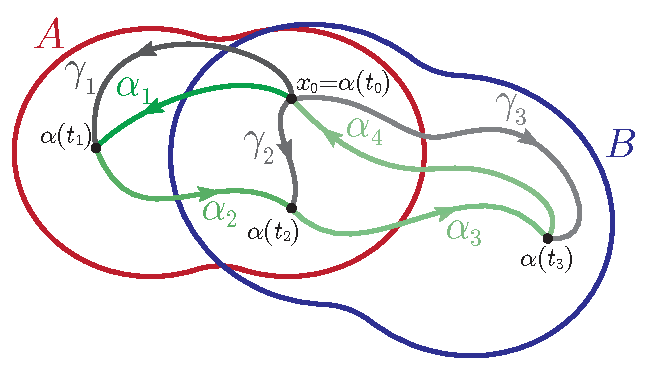
\includegraphics[trim=0cm 0cm 0cm 0.2cm,clip,scale=0.7]{images/vankampenpaths.pdf}
	\end{center}
		\vspace{-6mm}
	Grazie a $\gamma_i$ ora si può ottenere un \textit{cammino chiuso}: $\forall i=1,\ \dots,\ k$ sia $\beta_i\coloneqq (\gamma_{i-1}\ast \alpha_i)\ast\overline{\gamma_i}$: è ben definito e, per costruzione, è un cammino chiuso con \textit{punto base} $x_0$, quindi segue che $[\beta_i]\in \homotopy[1]{X,x_0}$. Mostriamo ora che $\img \beta_i$ è contenuta o in $A$ o in $B$. Fissato $i\in\left\{1,\ \dots,\ k\right\}, \ \img\alpha_i=\alpha([t_{i-1},\ t_i])$ è contenuto o in $A$ o in $B$, osserviamo che
		\begin{equation*}
			\begin{array}{llll}
				&\img\alpha_i \subseteq A &\implies \alpha(t_{i-1})\in A,\ \alpha(t_i)\in A &\implies \gamma_{i-1} \text{ e } \gamma_i \text{ entrambi a valori in }A \\
				&\implies \img\beta_i \subseteq A &\implies [\beta_i]\in G_A&\\
			\end{array}
		\end{equation*}
	In modo analogo si può mostrare da $\img\alpha_i \subseteq B$ che $[\beta_i]\in G_B$. Quindi $[\beta_i]\in G_A\cup G_B,\ \forall i$ e
	\begin{equation*}
		[\alpha]=[\alpha_1 \ast \dots \ast\alpha_k]=[\beta_1\ast\dots\ast\beta_k]=[\beta_1]\cdots [\beta_k],
	\end{equation*}
pertanto $G_A\cup G_B$ generano $\homotopy[1]{X,x_0}$.\qedhere
\end{proof}
\begin{corollary}{}[$X$ dato da due aperti semplicemente connessi non disgiunti è semplicemente connesso; Manetti, 11.26]\label{corollario Van Kampen}
Sia $X$ uno spazio topologico e siano $A,\ B\subseteq X$ aperti tali che:
		\begin{enumerate}
			\item $A$ e $B$ sono \textit{semplicemente connessi};
			\item $A\cap B\neq\emptyset$ è c.p.a.;
			\item $X=A\cup B$.
		\end{enumerate}
	Allora $X$ è \textit{semplicemente connesso}.
\end{corollary}
\begin{proof}{n}
	Per il teorema \ref{unionecpa} $X$ è c.p.a., essendo unione di c.p.a. con intersezione non vuota. Siccome l'intersezione non è vuota, sia $x_0\in A\cap B$: le ipotesi del \textit{teorema di Van Kampen} appena dimostrato sono soddisfatte, quindi $\homotopy[1]{X,x_0}$ è generato da $G_A$ e $G_B$. Tuttavia $A$ è semplicemente connesso, dunque $\homotopy[1]{A,x_0}=\left\{1\right\}$; considerando $
		\funct{s}[i_\ast]{\homotopy[1]{A,x_0}}{G_A}$ suriettiva, $G_A=\left\{1\right\}$ e, con procedimento analogo, si vede che $G_B=\left\{1\right\}$. Siccome $\homotopy[1]{X,x_0}$ è generato da $G_A\cup G_B=\left\{1\right\}$, allora $\homotopy[1]{X,x_0}=\left\{1\right\}$.
\end{proof}
\section{Gruppo fondamentale della sfera}
\begin{remark}{}[Proiezione stereografica]
	Si ha che $\forall p\in S^n,\ S^n\setminus \{1\text{ punto}\}\cong \R^n$ tramite la \textbf{proiezione stereografica}\index{proiezione!stereografica}. Per definirla, si consideri la \textit{sfera} $S^n$ centrata nell'origine e privata del punto $N=(0,\ 0,\ \ldots,\ 1)$, detto \textbf{polo Nord} \index{polo Nord}: la proiezione stereografica sarà la mappa
	\begin{equation*}
		\funct{}[\pi]{S^n\setminus\{N\}}{H\coloneqq\left\{\left(x_0,\ \ldots,\ x_n\right)\in\R^{n+1}\mid x_n=0\right\}}
	\end{equation*}
	che al punto $Q\in S^n$ associa l'intersezione $\pi\left(Q\right)$ della \textit{retta} per $N$ e $Q$ con l'iperpiano $H$.
	\begin{center}
	\includegraphics[trim=0cm 0cm 0cm 0cm,clip,scale=0.7]{images/stereo.pdf}
	\end{center}
	 La proiezione stereografica\footnote{Nelle ‘‘Note aggiuntive'', a pag. \pageref{proiezionestereograficanote}, si può trovare la proiezione stereografica per $n=2$.} è in particolare un \textit{omeomorfismo} e, poiché $H\cong\R^n$ (in quanto iperpiano di $\R^{n+1}$), si ha $S^n\setminus \{1\text{ punto}\}\cong \R^n$.
\end{remark}
\begin{corollary}{n}[$S^n$ è semplicemente connessa, $\forall n\geq 2$; Manetti, 11.27] \label{sfere sempl. connesse}
\end{corollary}
\begin{proof}{n}
	Applichiamo il \textit{teorema di Van Kampen}, scegliendo degli aperti adatti. Sia:
	\begin{itemize}
		\item $N=(0,\ \dots,\ 0,\ 1)\in S^n$ il polo Nord.
		\item $S=(0,\ \dots,\ \ -1)\in S^n$ il polo Sud\index{polo Sud}.
	\end{itemize}
	Definiamo $A\coloneqq S^n\setminus\{N\}$: esso è aperto, c.p.a., omeomorfo a $\R^n$ per la \textit{proiezione stereografica} e, siccome $\R^n$ è contraibile, lo è anche $A$; dunque sarà \textit{semplicemente connesso}. Lo stesso è vero per $B\coloneqq S^n\setminus\{S\}$. Si ha $A\cap B=S^n\setminus\{N, S\}$ c.p.a. se $n\geq 2$, $A\cap B$ è \textit{non} vuoto e inoltre $S^n=A\cup B$; per il corollario \ref{corollario Van Kampen} si ha che $S^n$ è \textit{semplicemente connesso}.
\end{proof}
\begin{warning}{n}
	$X$ \textit{contraibile} implica $X$ \textit{semplicemente connesso}, ma \textit{non} vale il viceversa! Infatti, le sfere $S^n, n\geq 2$ sono \textit{semplicemente connesse} ma \textit{non} sono contraibili perché \textit{non} sono omotopicamente equivalenti ad un \textit{punto}. Pertanto, il tipo di omotopia di $X$ determina il gruppo fondamentale di $X$, ma non vale il viceversa!
\end{warning}
\section{Gruppo fondamentale della circonferenza}
Nella sezione precedente abbiamo analizzato il gruppo fondamentale delle sfere $S^n$ per $n\geq 2$: ci domandiamo ora cosa succede per la circonferenza $S^1$. Siccome la dimostrazione\footnote{Per la dimostrazione del teorema seguiremo il capitolo 16 di \cite{kosniowski:1980firstlook}.} sarà lunga e articolata, preannunciamo che il gruppo fondamentale che otterremo \textit{non} è banale, ma è $\homotopy[1]{S^1}\cong \Z$: nello specifico, l'isomorfismo rappresenta il \textit{numero di giri} con \textit{segno} che un cammino chiuso fa \textit{intorno} alla circonferenza. Dunque, la nostra intenzione è di formalizzare il concetto che ogni intervallo fra due interi consecutivi ‘‘\textit{copre}'' la circonferenza.
\begin{center}
	\includegraphics[width=240pt]{images/slinky-eps-converted-to.pdf}
\end{center}
\subsection{Mappa esponenziale}
\begin{definition}{}[Mappa esponenziale]
La \textbf{mappa esponenziale}\index{mappa esponenziale} si può considerare come proiezione ad un quoziente per l'azione di $\Z$ su $\R$, cioè è la seguente funzione continua e \textit{aperta}:
	\begin{equation*}
		\funct{}[e]{\R}{S^1}[t][e^{2\pi i t}]
	\end{equation*}
Con questa notazione si considera $S^1\subseteq\C$, per cui $S^1=\Set{z\in\C | \abs{z}=1 }$.\footnote{Si veda a riguardo la digressione a pag. \pageref{complessir2}.}
\end{definition}
Utilizzeremo come punto base per i nostri scopi il punto $(1,0) \in \R^2$, equivalente a $1\in\C$.
\subsubsection{Rivestimento}
Vogliamo ora utilizzare questa proprietà per definire il numero di giri che fa un cammino chiuso intorno alla circonferenza.
\begin{lemma}{}[Aperto uniformemente rivestito di $S^1$]\label{teo uniformemente rivestito}
Sia $U\subsetneqq S^1$ aperto. Allora
	\begin{equation*}
		e^{-1}(U) = \coprod_{n\in\Z} V_n
	\end{equation*}
con $V_n\subseteq\R$ aperto; la restrizione $\funct{}[e_{\mid_{V_n}}]{V_n}{U}$ è un omeomorfismo $\forall n\in\Z$.
\end{lemma}
\begin{definition}{}[Uniformemente rivestito]
	Un tale $U$ aperto di un qualsiasi spazio topologico $X$ si dice \textbf{uniformemente rivestito}.\index{uniformemente rivestito}
\end{definition}
\begin{proof}{n}
	Si consideri un punto \textit{non} in $U$, ad esempio supponiamo $1\notin U$. Si ha
	\begin{equation*}
		e^{-1}(1)=\{t\in\R \mid e^{2\pi i t}=\cos(2\pi t)+i\sin(2\pi t)=1\}=\Z \implies \Z \cap e^{-1}(U)=\emptyset
	\end{equation*}
	Dunque, $\Z$ è \textit{disgiunto} dalla controimmagine di $U$. Poniamo ora $V_0\coloneqq e^{-1}(U)\cap \unint= e^{-1}(U)\cap (0,\ 1)$, in quanto la controimmagine di $U$ non contiene interi.\\
		\begin{minipage}[t]{0.68\textwidth}
	\begin{itemize}
	\item $V_0$ è aperto in $\R$ in quanto intersezione di aperti.
	\item La restrizione $e_{\mid_{V_0}}$ è iniettiva.
	\item $e(V_0)=U$ in quanto $e\left( (0,\ 1) \right)=S^1\setminus\left\{1\right\}$ e $U\subseteq S^1\setminus\left\{1\right\}$ per ipotesi.
\end{itemize}
Siccome $e$ è \textit{aperta}, la restrizione $\funct{}[e_{\mid_{V_0}}]{V_0}{U}$ è un \textit{omeomorfismo} in quanto è biunivoca, continua e aperta. Definiamo ora $V_n\coloneqq V_0 +n=\{ x+n \mid x\in V_0\},\ \forall n\in\Z$. Allora:
\begin{equation*}
	e^{-1}(U)=\bigcup_{n\in\Z} V_n\text{ e }V_n\subseteq (n,\ n+1)
\end{equation*}
Quindi $V_n\cap V_m=\emptyset$ se $n\neq m$, che implica l'\textit{iniettività} della funzione $e_{\mid_{V_n}}$ e il fatto che la somma di sopra sia \textit{disgiunta}. Essendo $e(V_n)=U$, allora $\funct{}[e_{\mid_{V_n}}]{V_n}{U}$ è un omeomorfismo.
	\end{minipage}
	\begin{minipage}[t]{0.31\textwidth}\vspace{-10pt}
	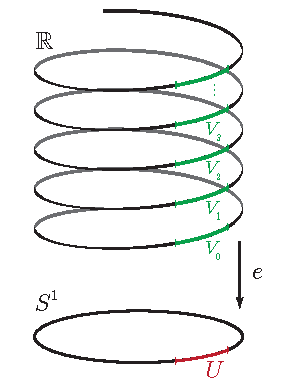
\includegraphics[trim=0cm 0cm 0cm 0cm,clip,scale=1]{images/spiralexponential.pdf}
	\end{minipage}
\end{proof}
\subsection{Sollevamento}
\begin{definition}{n}[Sollevamento]~{}\\
	\begin{minipage}[t]{0.78\textwidth}
		Sia $\alpha$ un cammino in $S^1$. Un \textbf{sollevamento}\index{sollevamento} di $\alpha$ è una funzione \textit{continua} $\funct {}[\widetilde{\alpha}]{I}{\R}$ tale che commuti il diagramma a lato, cioè tale che $\alpha= e\circ \widetilde{\alpha}$. Più in generale, dato $X$ spazio topologico e $\funct{}[f]{X}{S^1}$ continua, un \textit{sollevamento} di $f$ è la funzione $\funct{}[\widetilde{f}]{X}{\R}$ continua tale che $f=e\circ \widetilde{f}$.
	\end{minipage}
	\begin{minipage}[t]{0.21\textwidth}\vspace{-10pt}
		\begin{tikzcd}
			&  & \R \arrow[dd, "e"] \\
			&  &                     \\
			I \arrow[rr, "\alpha"] \arrow[rruu, "\widetilde{\alpha}" , dashed] &  & S^1
		\end{tikzcd}
	\end{minipage}
\end{definition}
Se $\widetilde{\alpha}$ è un sollevamento di $\alpha$, allora:
	\begin{equation*}
		\forall t\in I, \ e(\widetilde{\alpha}(t))=\alpha(t)\implies e^{2\pi i \widetilde{\alpha}(t)}=\cos(2\pi \widetilde{\alpha}(t))+i\sin(2\pi\widetilde{\alpha}(t))=\alpha(t)
	\end{equation*}
Dunque $2\pi\widetilde{\alpha}(t)$ è una \textit{determinazione dell'angolo} per $\alpha(t)\in S^1$; muovendosi con continuità su $S^1$ tramite $\alpha$ ci si muove in maniera continua anche tramite $\widetilde{\alpha}$, ossia $2\pi\widetilde{\alpha}$ è una \textbf{determinazione continua}\index{determinazione continua} dell'angolo per $\alpha$.
\begin{example}{n}
	Fissato $n\in\Z$, si consideri il cammino:
	\begin{equation*}
		\funct{}[\gamma]{I}{S^1}[t][e^{2\pi i nt}]
	\end{equation*}
	Ad esempio, per $n=1$ si percorre un giro in senso \textit{antiorario}, con $n=2$ si percorrono due giri in senso antiorario, con $n=-1$ si percorre un giro in senso \textit{orario}. Un sollevamento di $\gamma$ è dato da $\funct{}[\widetilde{y}]{I}{\R}$ con $\gamma(t)=e(\widetilde{\gamma}(t))$. Poiché $\gamma$ è già scritto in forma esponenziale, si ha $\widetilde{\gamma}(t)=nt$.
\end{example}
Andiamo ora a verificare l'\textit{esistenza} di sollevamenti per cammini e vedere se e quando sono \textit{unici}.
\begin{theorem}{}[Sollevamento di cammini]\label{teo sollevamento cammini}
Ogni cammino $\funct{}[\alpha]{I}{S^1}$ ammette un sollevamento $\funct{}[\widetilde{\alpha}]{I}{\R}$. Inoltre, fissato il punto iniziale, il sollevamento è \textit{unico}: fissato $x_0\in\R$ tale che $e(x_0)=\alpha(0)$, ossia $x_0\in e^{-1}(\alpha(0))$ fibra di $\alpha(0)\in S^1$, esiste ed è unico $\funct{}[\widetilde{\alpha}]{I}{\R}$ sollevamento di $\alpha$ \textit{a partire da} $x_0$, cioè $\widetilde{\alpha}(0)=x_0$.
\end{theorem}
\begin{proof}{n}~{}
	\begin{itemize}
		\item \textbf{Esistenza}: Per dimostrare l'\textit{esistenza} si considerano degli aperti \textit{uniformemente rivestiti}, dividendo $I$ in modo tale da avere sottointervalli la cui immagine tramite $\alpha$ sia contenuta in un \textit{aperto rivestito}; costruiremo induttivamente il sollevamento ‘‘a pezzi'', componendo con le inverse locali dell'esponenziale. Per ogni $p\in S^1$ punto della circonferenza, sia $U_p\subsetneqq S^1$ un intorno aperto \textit{connesso} di $p$. Allora $U_p$ è \textit{uniformemente rivestito} e $\{U_p\}_{p\in S^1}$ è un ricoprimento aperto di $S^1$. Sia $\funct{}[\alpha]{I}{S^1}$ un cammino; per il corollario \ref{corollario suddivisione} del \textit{teorema di Lebesgue} si ha che esiste una suddivisione $0=t_0\leq t_1\leq\dots\leq t_k=1$ tale che
		\begin{equation*}
			\forall i=1,\ \dots,\  k,\ \alpha([t_{i-1},\ t_i])\subseteq U_i\text{ aperto del ricoprimento.}
		\end{equation*}
		Costruiamo ora il sollevamento ‘‘a pezzi'' \textit{induttivamente} su ciascun intervallino $[0,\ t_i]$: prima si costruisce il passo base per $[0,\ t_1]$ poi, assumendo di aver già definito il sollevamento fino a $t_i$, lo si costruisce fino a $t_{i+1}$.\\
		\begin{itemize}
			\item[$\underline{t_1}$] Posto $\widetilde{\alpha}(0)=x_0$, per $[0,\ t_1]$ si ha che $\alpha\left([0,\ t_1]\right)\subseteq U_1$ uniformemente rivestito; pertanto, per il lemma \ref{teo uniformemente rivestito} (pag. \pageref{teo uniformemente rivestito}) vale
			\begin{equation*}
				 e^{-1}(U_1) = \coprod_{n\in\Z}V_n\text{ aperto in } \R\ \text{tale che}\ \funct{}[e_{\mid_{V_n}}]{V_n}{U_1} \text{ è omeomorfismo.}
			\end{equation*}
			Siccome $x_0\in e^{-1}(\alpha(0))$ e $\alpha(0)\in U_1$ allora $x_0\in e^{-1}(U_1)$. Tuttavia, i $V_n$ sono disgiunti, quindi esiste unico $\overline{n}$ per cui $x_0\in V_{\overline{n}}$. Siccome $\funct{}[e_{\mid_{V_{\overline{n}}}}]{V_{\overline{n}}}{U_1}$ è un omeomorfismo, allora ha un'inversa locale
			\begin{equation*}
				\funct{}[\phi\coloneqq \left(e_{\mid_{V_{\overline{n}}}}\right)^{-1}]{U_1}{V_{\overline{n}}}.
			\end{equation*}
			Poniamo ora come primo ‘‘pezzo'' del sollevamento:
			\begin{equation*}
				\widetilde{\alpha_1}\coloneqq \phi\circ \alpha_{\mid_{[0,\ t_1]}},\ \funct{}[\widetilde{\alpha_1}]{[0,\ t_1]}{\R}
			\end{equation*}
		\item[$\underline{t_{i+1}}$] Supponiamo di avere definito $\funct{}[\widetilde{\alpha_i}]{[0,\ t_i]}{\R}$ continua, sollevamento di $\alpha_{\mid_{[0,\ t_i]}}$, ossia il sollevamento di $\alpha$ da $0$ fino a $t_i$. Procedendo analogamente al primo intervallo: consideriamo $\alpha\left( [t_i,\ t_{i+1}] \right)\subseteq U_{i+1}$ uniformemente rivestito, tale per cui
		\begin{equation*}
			 e^{-1}(U_{i+1})=\coprod_{m\in\Z} W_m
		\end{equation*}
		con $W_m$ aperti. Fra questi $W_m$ scegliamo quello che contiene il punto di partenza.
		\begin{equation*}
			\widetilde{\alpha_i}(t_i)\in e^{-1}\left( \alpha(t_i) \right) \implies \widetilde{\alpha_i}(t_i)\in e^{-1}\left( U_{i+1} \right) \implies \exists ! \overline{m} \colon \widetilde{\alpha_i}(t_i)\in W_{\overline{m}}.
		\end{equation*}
	Sia
	\begin{equation*}
		\funct{}[\psi\coloneqq \left( e_{\mid_{W_{\overline{m}}}} \right)^{-1}]{U_{i+1}}{W_{\overline{m}}}
	\end{equation*}
	e poniamo $\funct{}[\widetilde{\alpha_{i+1}}]{[0,\ t_{i+1}]}{\R}$ inversa locale che estende il sollevamento $\widetilde{\alpha_i}$ come segue:
	\begin{equation*}
		\widetilde{\alpha_{i+1}}(t)= \begin{cases}
			\widetilde{\alpha_i}(t) & t\in [0,\ t_i]\\
			\psi\circ \alpha(t) & t\in[t_i,\ t_{i+1}]
		\end{cases}
	\end{equation*}
		Tale funzione è continua per il lemma di incollamento \ref{lemmaincollamento}.
		\end{itemize}
	Procedendo in questo modo definiamo $\funct{}[\widetilde{\alpha}]{\unint}{\R}$ sollevamento di $\alpha$ a partire da $x_0$.
	\item \textbf{Unicità}: Sia $\funct{}[\widehat{\alpha}]{\unint}{\R}$ un \textit{altro} sollevamento di $\alpha$ a partire da $x_0$. Sia $Y$ l'insieme dove $\widetilde{\alpha}$ e $\widehat{\alpha}$ coincidono:
	\begin{equation*}
		Y \coloneqq \{t\in I \mid \widetilde{\alpha}(t)=\widehat{\alpha}(t)\}
	\end{equation*}
	Allora:
	\begin{itemize}
		\item $0\in Y \implies Y\neq\emptyset$ dato che $\widetilde{\alpha}(0)=\widehat{\alpha}(0)=x_0$.
		\item $Y$ è chiuso in quanto luogo dei punti su cui coincidono due mappe continue a valori in uno spazio di \textbf{Hausdorff}.
	\end{itemize}
	Mostriamo che $Y$ è anche \textit{aperto}, così per la connessione di $I$ si ha che $Y=I$, il che implica $\widetilde{\alpha}=\widehat{\alpha}$. Per dimostrare che $Y$ è aperto dimostriamo che è intorno di ogni suo punto, usando gli intorni uniformemente rivestiti. Sia $t_0\in Y$ e sia $\alpha(t_0)\in S^1$. Sia $U$ un intorno aperto di $\alpha(t_0)$ uniformemente rivestito; si ha
	\begin{equation*}
		 e^{-1}(U)=\coprod_{n\in\Z}V_n
	\end{equation*}
	e vale inoltre
	\begin{equation*}
		\widetilde{\alpha}(t_0)=\widehat{\alpha}(t_0)\in e^{-1} \left( \alpha(t_0) \right)\subseteq e^{-1}(U)
	\end{equation*}
	Per il lemma \ref{teo uniformemente rivestito} (pag. \pageref{teo uniformemente rivestito}) esiste ed è unico $\overline{n}$ tale che $\widetilde{\alpha} (t_0)=\widehat{\alpha}(t_0)\in V_{\overline{n}}$ aperto in $\R$. Poniamo $A\coloneqq \widetilde{\alpha}^{-1}(V_{\overline{n}}) \cap \widehat{\alpha}^{-1}(V_{\overline{n}})$. Si ha:
	\begin{itemize}
		\item $A$ è aperto in $I$ in quanto intersezione di controimmagine tramite funzioni continue di aperti.
		\item $t_0 \in A$.
	\end{itemize}
	Mostriamo ora che le due funzioni coincidano su $A$, ossia $\widetilde{\alpha}(t)=\widehat{\alpha}(t),\ \forall t\in A$. Se $t\in A$, per definizione di $A$ si ha che $\widetilde{\alpha}(t)$ e $\widehat{\alpha}(t)\in V_{\overline{n}}$, dunque per definizione di sollevamento
	\begin{equation*}
		e\left( \widetilde{\alpha}(t) \right)= e\left( \widehat{\alpha}(t) \right)= \alpha(t).
	\end{equation*}
	Ma $e_{\mid_{V_{\overline{n}}}}$ è iniettiva perché è un omeomorfismo, quindi se $\widetilde{\alpha}(t)=\widehat{\alpha}(t)$ si ha $A\subseteq Y$ e dunque $t_0$ è interno a $Y$. Per l'arbitrarietà di $t_0$ vale $Y$ aperto.
	\end{itemize}
\end{proof}
\subsubsection{Grado di un cammino}
\begin{definition}{}[Grado di un cammino chiuso in $S^1$]
	Sia $\funct{}[\alpha]{I}{S^1}$ un cammino chiuso con punto base $1\in S^1$ e sia $\funct{}[\widetilde{\alpha}]{I}{\R}$ l'unico sollevamento di $\alpha$ a partire da $x_0=0 \in e^{-1} (1)$. Si definisce \textbf{grado}\index{grado} di $\alpha$ come il punto finale del sollevamento:
	\begin{equation*}
		\deg (\alpha)\coloneqq \widetilde{\alpha}(1).
	\end{equation*}
\end{definition}

\begin{remark}{}[{$\deg(\alpha)\in\Z$}]% $\circled{1}\quad$ \textsc{$\deg(\alpha)\in\Z$.}\\
	Quella appena data è una \textit{buona definizione} grazie al teorema precedente, che assicura che il sollevamento esiste ed è unico.	Inoltre $\deg(\alpha)\in\Z$: per definizione di sollevamento, siccome il cammino è chiuso
	\begin{equation*}
		\widetilde{\alpha}(1)\in e^{-1}(\alpha(1))=e^{-1}(\alpha(0))=e^{-1}(1)=\Z.
	\end{equation*}
	Il grado conta il \textbf{numero di giri} con \textit{segno} di $\alpha$ intorno a $S^1$, dove il segno è \textit{positivo} se gira in senso \textit{antiorario}, e \textit{negativo} se gira in senso \textit{orario}.
\end{remark}
Abbiamo così formalizzato il numero di giri con segno intorno a $S^1$.
\begin{example}{pn}~{}
	\begin{itemize}
		\item Sia $\alpha(t)=e^{2\pi i t}$, con $t\in\unint$, e sia $\widetilde{\alpha}(t)=t$ il sollevamento di $\alpha$ a partire da $x_0=0$. Siccome $\widetilde{\alpha}(1)=1$, allora $\deg\alpha=1$, quindi $\alpha$ percorre solo un giro in senso antiorario intorno a $S^1$.
		\item Fissato $n\in\Z$, sia
		\begin{equation*}
			\funct{}[\gamma]{I}{S^1}[t][e^{2\pi i nt}].
		\end{equation*}
		Esso è un cammino chiuso con punto base $1$. Il sollevamento di $\gamma$ con punto base $x_0=0$ è dato da $\widetilde{\gamma}(t)=nt$, dunque $\deg\gamma=\widetilde{\gamma}(1)=n$.
	\end{itemize}
\end{example}

\begin{remark}{}[{$\deg\alpha$ con punto base arbitrario}] %$\circled{2}\quad$ \textsc\\
	Sia $\funct{}[\alpha]{I}{S^1}$ un cammino chiuso con punto base $1$, $\widetilde{\alpha_0}$ il sollevamento di $\alpha$ con punto base $x_0=0$. Preso $n\in\Z$, si consideri $\funct{}[\widetilde{\alpha_n}]{I}{\R}$ definita come $\widetilde{\alpha_n}=\widetilde{\alpha_0}+n$. Siccome per ogni punto nella \textit{fibra} del punto iniziale esiste ed è unico il \textit{sollevamento}, e siccome la fibra in questo caso è $\Z$ si ha che, per ogni intero, il sollevamento sarà il traslato di $\widetilde{\alpha_0}$. Per mostrarlo, osserviamo che $\widetilde{\alpha_n}$ è continuo ed è un sollevamento di $\alpha$, infatti
		\begin{equation*}
			e\left( \widetilde{\alpha_n}(t) \right)= e^{2\pi i \widetilde{\alpha_n}(t)}= e^{2\pi i (\widetilde{\alpha_0}(t)+n)}=e^{2\pi i \widetilde{\alpha_0}(t)} e^{2\pi i n}=\alpha(t)
		\end{equation*}
	Il suo punto iniziale è $n$, infatti $\widetilde{\alpha_n}(0)=\widetilde{\alpha_0}(0)+n=n$.	Quindi $\widetilde{\alpha_n}$ è il sollevamento di $\alpha$ a partire da $x_0=n$. Inoltre,
		\begin{equation*}
			\widetilde{\alpha_n}(1)- \widetilde{\alpha_n}(0)=\widetilde{\alpha_0}(1)+n - (\underbrace{\widetilde{\alpha_0}(0)}_{=0}+n)= \widetilde{\alpha_0}(1)=\deg\alpha.
		\end{equation*}
	Pertanto $\deg\alpha= \widetilde{\alpha}(1)-\widetilde{\alpha}(0)$ con $\widetilde{\alpha}$ un sollevamento qualsiasi.	Si può quindi riformulare la definizione di grado di un cammino chiuso $\alpha$ in $S^1$ con \textit{punto base qualsiasi} come la differenza fra il punto finale e quello iniziale di un sollevamento $\widetilde{\alpha}$ \textit{qualsiasi} del cammino:
	\begin{equation*}
		\deg (\alpha)\coloneqq \widetilde{\alpha}(1)-\widetilde{\alpha}(0).
	\end{equation*}
\end{remark}
Vediamo ora come si comporta il grado rispetto al prodotto di cammini.
\begin{theorem}{}[Grado del prodotto di cammini è somma dei gradi]
	Siano $\alpha,\ \beta$ cammini chiusi in $S^1$ con punto base $1$. Allora
	\begin{equation*}
		\deg(\alpha\ast\beta)=\deg\alpha + \deg\beta.
	\end{equation*}
\end{theorem}
\begin{proof}{n}
	Sia $\widetilde{\alpha}$ il sollevamento di $\alpha$ a partire da $x_0=0$. Allora definiamo $a\coloneqq \widetilde{\alpha}(1)=\deg\alpha\in\Z$. Sia $\widehat{\beta}$ il sollevamento di $\beta$ a partire da $a$; si ha:
	\begin{equation*}
		\deg\beta=\widehat{\beta}(1)-\widehat{\beta}(0)=\widehat{\beta}(1)-a
	\end{equation*}
	Siccome $\widetilde{\alpha}(1)=\widehat{\beta}(0)$ si può considerare il cammino congiunto $\funct{}[\widetilde{\alpha}\ast\widehat{\beta}]{I}{\R}$. Dimostriamo che è un sollevamento di $\alpha\ast\beta$:
		\begin{gather*}
			e\left( \widetilde{\alpha}\ast\widehat{\beta}(t) \right)= e^{2\pi i \widetilde{\alpha}\ast\widehat{\beta}(t)}=\begin{cases}
				e^{2\pi i \widetilde{\alpha}(t)}, & t\in \left[ 0,\ \frac{1}{2} \right]\\
				e^{2\pi i \widehat{\beta}(2t-1)}, & t\in \left[ \frac{1}{2},\ 1 \right]
			\end{cases}=\begin{cases}
				\alpha(2t), & t\in \left[ 0,\ \frac{1}{2} \right]\\
				\beta(2t-1), & t\in \left[ \frac{1}{2},\ 1 \right]
			\end{cases}= \alpha\ast\beta(t)\\
			(\widetilde{\alpha}\ast\widehat{\beta})(0)=\widetilde{\alpha}(0)=0 \implies \deg(\alpha\ast\beta)=(\widetilde{\alpha}\ast\widehat{\beta})(1)=\widehat{\beta}(1)=a+\deg\beta=\deg\alpha +\deg\beta\qedhere
		\end{gather*}
\end{proof}
Si può dimostrare, anche se in questa sede non lo faremo, che il grado è \textit{invariante} per omotopia di cammini; concettualmente consiste nel costruire un sollevamento fra le omotopie per mostrare che hanno lo stesso grado.
\begin{theorem}{q}[Teorema di monodromia]
	Siano $\alpha,\ \beta$ cammini chiusi in $S^1$ con punto base $1$ e supponiamo che $\alpha$ e $\beta$ siano cammini omotopi. Allora $\deg\alpha=\deg\beta$, cioè il grado è invariante per omotopia di cammini.\qedhere
\end{theorem}

\subsection{Dimostrazione del gruppo fondamentale della circonferenza}
\begin{theorem}{}[Gruppo fondamentale di $S^1$]
	\begin{equation*}
		\homotopy[1]{S^1,1}\cong\Z
	\end{equation*}
\end{theorem}
\begin{proof}{n}
	Sia
	\begin{equation*}
	\funct{}[\Phi]{\homotopy[1]{S^1,1}}{\Z}[\left[\alpha\right]][\deg\alpha].
	\end{equation*}
	Vogliamo dimostrare che è un \textit{isomorfismo di gruppi} per ottenere la tesi.
		\begin{itemize}
			\item $\Phi$ è un'applicazione \textit{ben definita} per il teorema di monodromia.
			\item $\Phi$ è un \textit{morfismo di gruppi}: dati $[\alpha],[\beta]\in\homotopy[1]{S^1,1}$ si ha che
				\begin{equation*}
					\Phi([\alpha]\cdot [\beta])=\Phi([\alpha\ast\beta])=\deg(\alpha\ast\beta)=\deg\alpha+\deg\beta=\Phi([\alpha])+\Phi([\beta])
				\end{equation*}
			\item $\Phi$ è \textit{suriettiva}: per ogni $n\in\Z$, esiste un cammino chiuso $\gamma$ in $S^1$ e di grado $n$, per cui $\Phi([\gamma])=n$.
			\item $\Phi$ è \textit{iniettiva}; per far ciò, mostriamo che $\ker\Phi$ è banale. Sia $[\alpha]\in\ker\Phi$, vogliamo dimostrare che $[\alpha]=[C_1]$, cioè $\alpha\sim C_1$ cammino costante in $S^1$. Per ipotesi $\deg\alpha=\Phi([\alpha])=0$, quindi consideriamo il sollevamento di $\alpha$ con punto base $x_0=0$. Si ha $\deg\alpha=\widetilde{\alpha}(1)=0$, cioè $\alpha$ è un cammino chiuso.	Siccome $\R$ è contraibile, allora è \textit{semplicemente connesso}, dunque $\homotopy[1]{\R,0}=\left\{1\right\}$ e $[\widetilde{\alpha}]\in\homotopy[1]{\R,0}=\left\{1\right\}$.
			Pertanto, $[\widetilde{\alpha}]=[C_0]$: esiste un'omotopia di cammini $\funct{}[F]{I\times I}{\R}$ fra $\widetilde{\alpha}$ e $C_0$. $F$ è continua e:
			\begin{equation*}
				\begin{cases}
					F(t,0)=\widetilde{\alpha}(t)\\
					F(t,1)=0
				\end{cases}\forall t\in I\ \ \text{e}\ \
				F(0,s)=F(1,s)=0,\ \forall s\in I.
			\end{equation*}
				Sia $\funct{}[G\coloneqq e\circ F]{I\times I}{S^1}$: $G$ è continua e vale che:
				\begin{equation*}
					\begin{cases}
						G(t,0)=e(F(t,0))=e(\widetilde{\alpha}(t))=\alpha(t)\\
						G(t,1)=e(F(t,1))=e(0)=1
					\end{cases},\forall t\in I\ \ \text{e}\ \ 
					G(0,s)=G(1,s)=1,\ \forall s\in I.
				\end{equation*}
			$G$ è un'omotopia di cammini fra $\alpha$ e $C_1$ in $S^1$, pertanto $\Phi$ iniettiva.\qedhere
		\end{itemize}
\end{proof}
\subsection{Alcune conseguenze del gruppo fondamentale della circonferenza}
Osserviamo ora, con un esempio sulla circonferenza, che il corollario \ref{corollario Van Kampen} \textit{non} vale se $A$ e $B$ \textit{non} sono \textit{aperti}.
\begin{example}{n}
	Siano $X=S^1,\ A=(S^1\cap\{y>0\})\cup \{(1,0)\}$ e $B=S^1\cap\{y\leq 0\}$: notiamo come non sono aperti in $X$.\\
\begin{minipage}{.81\linewidth}
\begin{itemize}
	\item $A\cong (0,\ 1]\subseteq \R$ convesso in $\R$, allora $A$ è contraibile e dunque semplicemente connesso.
	\item $B=S^1\cap\{y\leq 0\}\cong\unint$ convesso in $\R$, allora $B$ è contraibile e dunque semplicemente connesso.
\end{itemize}
Si ha che $X=A\cup B,\ A\cap B=\{(1,\ 0)\}\neq\emptyset$ e c.p.a., ma $X=S^1$ come abbiamo appena dimostrato \textit{non} è semplicemente connesso!
	\end{minipage}
	\begin{minipage}{.18\linewidth}\vspace{-6mm}
		\includegraphics[trim=0cm 0cm 0cm 0cm,clip,scale=0.6]{images/notvankampen.pdf}
	\end{minipage}
\end{example}
\begin{corollary}{}[Circonferenza non è retratto del disco; Manetti, 12.38]\label{circonferenza non retratto disco}
Sia $D\subseteq\R^2$ il \textit{disco unitario} e $A=\partial{D}$ il suo \textit{bordo}, ossia $A=S^1$. Allora $A$ non è un retratto di $D$.
\end{corollary}
\begin{proof}{n}
	Se $A$ fosse un retratto, allora $\homotopy[1]{A}$ dovrebbe essere isomorfo ad un sottogruppo di $\homotopy[1]{D}$ perché l'inclusione induce un omomorfismo iniettivo (per il corollario \ref{grp fond iniettiva e suriettiva}, pag. \pageref{grp fond iniettiva e suriettiva}). Tuttavia, $\homotopy[1]{A}\cong\homotopy[1]{S^1}\cong\Z$ e $D\subseteq\R^2$ convesso fa si che $\homotopy[1]{D}\cong\left\{1\right\}$, il che è un assurdo in quanto $\Z\nleq \left\{1\right\}$!.\qedhere
\end{proof}
\begin{remark}{n}
	Allo stesso modo, se $X$ è uno spazio topologico \textit{semplicemente connesso} e $A\subseteq X$ con $A\cong S^1$, allora $A$ \textit{non} può essere un retratto di $X$.
\end{remark}

\begin{corollary}{}[Teorema del punto fisso di Brouwer; Manetti, 12.39]\label{punto fisso B}\index{punto fisso}\index{teorema!del punto fisso di Brouwer}
Sia $D\subseteq \R^2$ il disco unitario e sia $\funct{}[f]{D}{D}$ continua. Allora $f$ ha un punto fisso, ossia esiste $x_0\in D$ tale che $f(x_0)=x_0$.
\end{corollary}
\begin{proof}{n}
	Per \textit{assurdo}, supponiamo che $f$ \textit{non} abbia punti fissi, ossia $f(x_0)\neq x_0,\ \forall x_0\in D$. Utilizziamo $f$ per costruire una retrazione che non può esistere topologicamente parlando.
	\begin{minipage}{.82\linewidth}
		 Sia $\funct{}[r]{D}{\partial{D}}$ \textit{retrazione} continua con $r_{\partial{D}}=Id_{\partial{D}}$ definita nel modo seguente: se $S$ la semiretta aperta uscente da $f(x)$, dunque escludendo il punto $f(x)$, e passante per $x\neq f(x)$ per ipotesi dell'assurdo, poniamo $r(x)\coloneqq S\cap\partial{D}$.
	\end{minipage}
\begin{minipage}{.17\linewidth}
	\includegraphics[trim=0cm 0cm 0cm 0cm,clip,scale=0.5]{images/brower.pdf}
\end{minipage}
Se $x\in\partial{D}$, allora $x=r(x)$, quindi $r_{\mid_{\partial{D}}}= Id_{\partial{D}}$, ossia $r$ retrazione, il che è \textit{assurdo} per il corollario precedente.\qedhere
\end{proof}
\subsubsection{Invarianza della dimensione}
Grazie al calcolo del gruppo fondamentale della circonferenza si riescono anche a dimostrare dei casi particolari del \textit{teorema di invarianza della dimensione} (che verrà affrontato nel corso di \textit{Topologia Algebrica}).
\begin{theorem}{q}[Teorema di invarianza della dimensione]\index{teorema!di invarianza della dimensione}
Siano $U\subseteq\R^n$ e $V\subseteq \R^m$ aperti. Se $U$ e $V$ sono omeomorfi allora $n=m$. Per contronominale, se $n\neq m$ allora $U$ e $V$ non sono omeomorfi.\qedhere
\end{theorem}
\begin{example}{n}
	Sia $U\subseteq\R^n$ aperto con $n\geq 2$. Allora $U$ \textit{non} è omeomorfo ad un aperto di $\R$. Per dimostrarlo basta considerare una palla $B$ in $\R^n$ ed un intervallo $I$ in $\R$ e togliere ad entrambe un punto: nel primo caso si ottiene ancora un \textit{connesso}, mentre nel secondo uno \textit{sconnesso}, dunque \textit{non} possono essere \textit{omeomorfi}.
\end{example}
\begin{theorem}{}[Aperti di $\R^n$ di $n\geq 3$ non sono omeomorfi ad aperti di $\R^2$]\label{invarianzadimensionen=2}
	Sia $U\subseteq\R^n$ aperto con $n\geq 3$. Allora $U$ \textit{non} è omeomorfo ad un aperto di $\R^2$.
\end{theorem}
\begin{proof}{n}
	Ragionando per assurdo, ipotizziamo che $U$ sia omeomorfo ad un aperto di $\R^2$. Sia $B\subseteq U$ una palla aperta di centro $p$, allora $B$ è omeomorfo ad un aperto $A$ di $\R^2$. Sia $q\in A$ il punto corrispondente a $p$ tramite l'omeomorfismo, dunque $B\setminus\{p\}$ è omeomorfo a $A\setminus\{q\}$, ma $B\setminus\{p\}$ ha lo stesso tipo di omotopia di $S^{n-1}$. Infatti, sia $S$ una sfera centrata in $p$ tale per cui $S\subset B$, si ha che $S\cong S^{n-1}$ e $S\subset B\setminus\{p\}$ è un \textit{retratto di deformazione}. Supponiamo per semplicità che $p=\mathbf{0}$; la retrazione è data da
	\begin{equation*}
		\funct{}[r]{B\setminus \{\mathbf{0}\}}{S}[x][R\frac{x}{\| x \|}]
	\end{equation*}
	con $R$ raggio di $S$. Segue che $A\setminus \{q\}$ ha lo stesso tipo di omotopia di $S^{n-1}, n\geq 3\implies n-1\geq 2\implies S^{n-1}$ è semplicemente connesso, cioè $A\setminus\{q\}$ è \textit{semplicemente connesso}. $A$ aperto implica l'esistenza di $C$ circonferenza centrata in $q$ tale che $C\subset A$. Si ha che $C$ è un retratto - ma in generale \textit{non} di \textit{deformazione}! - di $A\setminus\{q\}$, sempre con la stessa retrazione di prima
	\begin{equation*}
		\funct{}[f]{A\setminus\{q\}}{C}[x=q+(x-q)][q+r(C)\frac{x-q}{\| x-q \|}]
	\end{equation*}
	con $r(C)$ raggio di $C$ e lo spostamento dovuto al fatto che $C$ è centrata in $q$. Se $x_0\in C\subset A\setminus\{q\}$, siccome esso è un retratto,  si ha che $\Z\cong \homotopy[1]{C,x_0}\leq\homotopy[1]{A\setminus\{q\},x_0}\cong\left\{1\right\}$, da cui l'assurdo.
\end{proof}
\begin{warning}{n}
	Non abbiamo potuto supporre che $A$ fosse una palla perché non sappiamo che ‘‘forma'' abbia dato l'omeomorfismo!
\end{warning}
\subsection{Gruppo fondamentale del prodotto}
\begin{theorem}{}[Gruppo fondamentale del prodotto; Manetti, 11.17]
	Siano $X$ e $Y$ spazi topologici, $x_0\in X$, $y_0\in Y$. Allora:
	\begin{equation*}
		\homotopy[1]{X\times Y,(x_0,y_0)}\cong \homotopy[1]{X,x_0}\oplus \homotopy[1]{Y,y_0}
	\end{equation*}
\end{theorem}
\begin{warning}{n}
	Con $\oplus$ si intende la \textit{somma diretta di gruppi}\index{somma!diretta di gruppi}, da intendersi nel caso di un numero \textit{finito} di gruppi come \textit{prodotto cartesiano}\index{prodotto!cartesiano} i cui morfismi sono \textit{componente per componente}. È diversa dalla \textit{somma diretta fra spazi vettoriali}, dato in quest'ultimo caso essa è un'operazione \textit{interna}!
\end{warning}
\begin{proof}{n}
	Un cammino $\funct{}[\alpha]{I}{X\times Y}$ è determinato dalle sue componenti $\alpha=(\alpha_1,\ \alpha_2)$ con $\funct{}[\alpha_1]{I}{X}$ e $\funct{}[\alpha_2]{I}{Y}$, dunque c'è la seguente corrispondenza biunivoca:
	\begin{equation*}
		\pathset{X\times Y}{(x_0,\ y_0),(x_0,\ y_0)}\leftrightarrow\pathset{X}{x_0,x_0}\times \pathset{Y}{y_0,y_0}.
	\end{equation*}
Allo stesso modo, la mappa $\funct{}[F]{I\times I}{X\times Y}$ è determinata dalle sue componenti $(F_1,\ F_2)$ con $ \funct{}[F_1]{I\times I}{X}$ e $\funct{}[F_2]{I\times I}{Y}$; inoltre, si ha che $F$ è omotopia fra i cammini $\alpha$ e $\beta$ se e solo se $F_i$ è un'omotopia di cammini fra $\alpha_i$ e $\beta_i$. Dunque c'è una corrispondenza biunivoca tra i quozienti:
\begin{gather*}
	\homotopy[1]{X\times Y,(x_0,y_0)}\leftrightarrow \homotopy[1]{X,x_0}\oplus \homotopy[1]{Y,y_0}\\
	[\alpha]\leftrightarrow ([\alpha_1],\ [\alpha_2])
\end{gather*}
Essa è anche un morfismo di gruppi, dato che $\alpha\ast\beta = (\alpha_1\ast\beta_1,\ \alpha_2\ast\beta_2)$: i gruppi sono isomorfi.\qedhere
\end{proof}
\section{Alcuni esempi di gruppi fondamentali}
\subsection{Toro}
\begin{definition}{}[Toro]\label{ciambella}
Il \textbf{toro}\index{toro} $T$ è lo spazio dato dal prodotto $S^1\times S^1$.
\end{definition}
	Siccome $S^1\subset\R^2$, si ha sicuramente che $T\subset \R^4$; tuttavia, esso è \textit{omeomorfo} al sottospazio $X$ di $\R^3$ che possiamo visualizzare come una ‘‘ciambella''.
	In particolare, si può definire come effetto della \textit{rotazione} attorno all'asse $z$ di una \textit{circonferenza} a esso disgiunta.\\
	\begin{minipage}{.42\linewidth}
		\begin{center}
				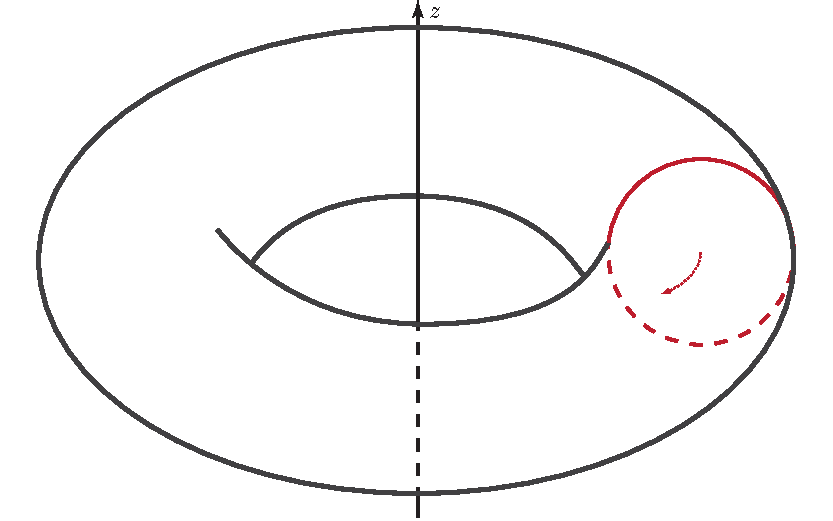
\includegraphics[trim=0cm 0cm 0cm 0cm,clip,scale=0.45]{images/torusalone.pdf}
		\end{center}
	\end{minipage}
	\begin{minipage}{.57\linewidth}
	Per il teorema precedente si ha
\begin{equation*}
	\homotopy[1]{T}=\homotopy[1]{S^1\times S^1}=\homotopy[1]{S^1}\oplus\homotopy[1]{S^1}=\Z\oplus\Z
\end{equation*}
Siccome $\Z$ è un gruppo \textit{ciclico infinito}, posso considerare per il gruppo fondamentale $\homotopy[1]{S^1}$ i generatori $\{-1\}$ e $\left\{1\right\}$, cioè la \textit{classe} del cappio di grado $1$ e quella di grado $-1$; si utilizzerà come generatore \textit{standard} $\gamma(t)=e^{2\pi i t}$.
	\end{minipage}\\
\begin{minipage}{.52\linewidth}
Per il toro, dunque, consideriamo i generatori corrispondenti a $(1,\ 0)$ e $(0,\ 1)$ in $\Z\oplus\Z$; scelto pertanto il punto base $x_0=(1,\ 1)$ si hanno:
\begin{itemize}
	\item $\alpha(t)=(e^{2\pi i t},\ 1)$, corrispondente ad un giro nel senso della circonferenza indicata in \textcolor{redill}{\textbf{rosso}}.
	\item $\beta(t)=(1,\ e^{2\pi i t})$, corrispondente ad un giro nel senso della circonferenza indicata in \textcolor{blueill}{\textbf{blu}}.
\end{itemize}
\end{minipage}
	\begin{minipage}{.47\linewidth}
		\begin{center}
				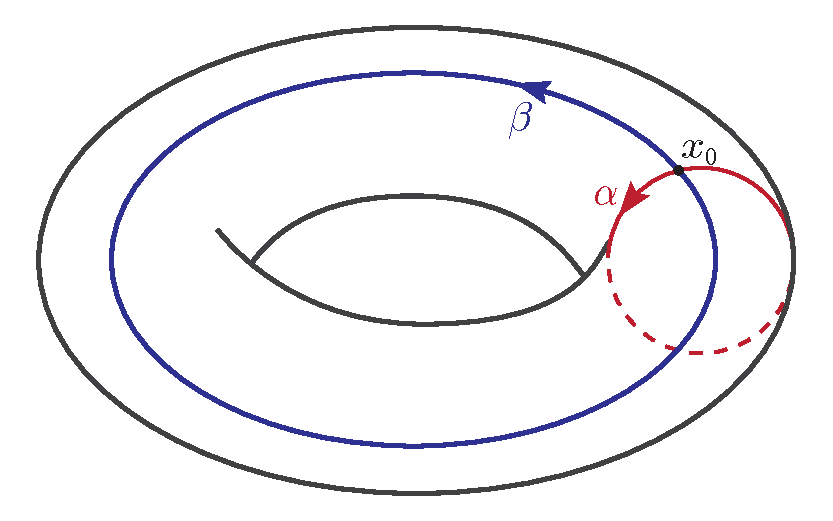
\includegraphics[trim=0cm 0cm 0cm 0cm,clip,scale=0.5]{images/torusgenerator.pdf}
		\end{center}
\end{minipage}
\subsection{Un gruppo fondamentale non abeliano}
% LEZ 21
Sia $X=S^1\vee S^1$ l'unione ad un punto di due circonferenze in $\R^2$, cioè il \textbf{bouquet di due circonferenze} che abbiamo trattato a pag. \pageref{bouquet}. Il gruppo fondamentale $\homotopy[1]{X,x_0}$ è il \textbf{gruppo libero}\footnote{Nelle ‘‘Note aggiuntive'', a pag. \pageref{gruppolibero}, si può trovare un approfondimento a riguardo.} $\Z\ast\Z$, i cui generatori sono due cammini $[\alpha]$ e $[\beta]$, uno per ciascuna circonferenza. Esso è \textit{infinito} e \textit{non abeliano} perché, preso ad esempio come punto base $x_0$, essi \textit{non} commutano, ossia $[\alpha\ast\beta]\neq [\beta\ast\alpha]$.
\subsection{Spazio proiettivo reale}
Consideriamo ora il caso dello \textit{spazio proiettivo reale}, che abbiamo introdotto nel capitolo \autoref{chap:azionidigruppo}. Ricordiamo la definizione \ref{def spazio proiettivo},
\begin{equation*}
	\Proj^n\left(\R\right)=\left(\R^{n+1}\setminus\{0\}\right)/\!\sim,
\end{equation*}
dove $x\sim y \iff \exists\lambda\in\R\setminus\{0\} \colon y=\lambda x$, cioè $\sim$ è la relazione indotta dall'azione di $\R\setminus\{0\}$ su $\R^{n+1}\setminus\{0\}$ per moltiplicazione. Ricordiamo inoltre la proposizione \ref{spazi proiettivi compatti connessi} per cui $\Proj^n\left(\R\right)$ è \textit{compatto} e \textit{connesso}; si ha inoltre che $\Proj^n\left(\R\right)$ è di \textbf{Hausdorff}. Considerata la \textit{restrizione} della proiezione $\funct{}[\pi_0\coloneqq \pi_{\mid_{S^n}}]{S^n}{\Proj^n\left(\R\right)}$, essa è continua, suriettiva e chiusa in quanto funzione da compatto in \textbf{Hausdorff}, quindi $\pi_0$ è un'identificazione. Pertanto, $\Proj^n\left(\R\right)$ è anche un quoziente di $S^n$ rispetto alla relazione che identifica i \textit{punti antipodali} $p$ e $-p$. Si consideri dunque la funzione associata, omeomorfismo di $S^n$:
\begin{equation*}
	\funct{}[\phi]{S^n}{S^n}[p][-p]
\end{equation*}
Tale relazione di equivalenza su $S^n$ è indotta dall'azione del gruppo $\{\pm 1\}$ per moltiplicazione, dunque $\funct{}[\pi_0]{S^n}{\Proj^n\left(\R\right)}$ è sia chiusa, sia aperta. In particolare, se $U\subset S^n$ è un aperto su cui $\pi_0$ è \textit{iniettiva}, allora $\funct{}[\pi_{0_{\mid_{S^n}}}]{U}{\pi_0(U)}$ è un \textit{omeomorfismo} perché continua, biunivoca e aperta. Da notare che, se $\pi_0$ è iniettiva su $U$, allora $U\subsetneqq S^n$; preso $p_0\in S^n$, se $U\subseteq S^n\setminus\{p_0\}\cong\R^n$ segue che $\pi_0(U)$ aperto in $\Proj^n\left(\R\right)$ è omeomorfo ad un aperto di $\R^n$. Analizziamo alcuni casi di dimensione \textit{bassa}:
	\begin{itemize}
		\item \underbfsf{$n=1$}: \textbf{retta proiettiva reale} $\Proj^1\left(\R\right)$.
		\item \underbfsf{$n=2$}: \textbf{piano proiettivo reale} $\Proj^2\left(\R\right)$. La sua descrizione geometrica esplicita può essere \textit{complicata}, tuttavia possiamo trovare un \textit{modello} che ci permetta di studiarlo comodamente. Data la mappa $\funct{}[\pi_0]{S^2}{\Proj^2\left(\R\right)}$ e considerata la \textit{calotta superiore} della sfera compreso l'\textit{equatore}, cioè $C\coloneqq S^2\cap\{z\geq 0\}$, si ha che $\pi_0(C)=\Proj^2\left(\R\right)$. Dunque, $\funct{}[\pi_{0_{\mid_{C}}}]{C}{\Proj^2\left(\R\right)}$ è ancora chiusa ed è ancora un'identificazione. Il piano proiettivo si può vedere come la calotta superiore con i \textit{punti antipodali dell'equatore} identificati.\\
\begin{minipage}{.23\linewidth}
	\includegraphics[trim=0cm 0cm 0cm 0cm,clip,scale=0.75]{images/projdisc.pdf}
\end{minipage}
\begin{minipage}{.76\linewidth}
	Sia ora $D\subset\R^2$ il disco unitario; si ha che $D\cong C$ tramite la proiezione ortogonale dei punti della calotta superiore sul piano $xy$, dunque $\funct{}{D}{\Proj^2\left(\R\right)}$ è un'identificazione che identifica i \textit{punti antipodali} su $\partial{D}$. Lo spazio quoziente che otteniamo su $D$ (e anche su $C$, chiaramente) è omeomorfo a $\Proj^2\left(\R\right)$ e prende il nome \textbf{modello piano di $\Proj^2\left(\R\right)$}.
\end{minipage}\\
		Da ciò si vede, anche intuitivamente, che il gruppo fondamentale risulta un gruppo di due elementi:
		\begin{equation*}
			\homotopy[1]{\Proj^2\left(\R\right),p_0}=\nicefrac{\Z}{2\Z}=\Z_2=\left\{\overline{0},\ \overline{1}\right\}
		\end{equation*}
	Vediamo il perché. Preso un punto base $p_0$:
		\begin{itemize}
				\item Qualunque cappio contenuto all'\textit{interno} del disco, cioè senza toccare alcun punto del bordo, è omotopicamente equivalente al cammino banale $C_0$ (e quindi la classe è $\left[C_0\right]$).
			\begin{center}
				\includegraphics[trim=0cm 0cm 0cm 0cm,clip,scale=0.95]{images/projdiscindisc.pdf}
			\end{center}
			\item Qualunque cappio che va ‘‘oltre il bordo'' \textit{una volta}, attraversando il cammino banale e torna indietro al punto base \textit{non} è banale. Infatti, non possiamo ridurre il cammino ad un cappio sul piano (dato che non avremmo più i punti sul bordo \textit{antipodali}), al più possiamo ‘‘ruotarlo'' attorno al punto base per ottenere un altro cappio omotopico al primo che attraversa sempre il bordo\footnote{Per semplicità, nelle figure abbiamo preso come punto il centro del disco. Questi ragionamenti e quelli successivi si adattano facilmente anche nel caso di un \textit{punto generico}, ponendo una leggera \textit{deformazione} al cappio in modo da fare rotazioni ‘‘lecite'', cioè che mantengono i punti del cammino posti sul bordo \textit{antipodali}.}.
						\begin{center}
				\includegraphics[trim=0cm 0cm 0cm 0cm,clip,scale=0.95]{images/projdiscoverborder1.pdf}
				\includegraphics[trim=0cm 0cm 0cm 0cm,clip,scale=0.95]{images/projdiscoverborder2.pdf}
				\includegraphics[trim=0cm 0cm 0cm 0cm,clip,scale=0.95]{images/projdiscoverborder3.pdf}
			\end{center}
		\end{itemize}
		Tuttavia, un cappio che va oltre il bordo \textit{due volte} è omotopicamente equivalente al cammino costante. Infatti, possiamo ‘‘ruotare'' la seconda parte del cappio (nell'immagine indicata con $3$ e $4$, cioè la parte del laccio dopo che ha già attraversato una volta il bordo) in modo da ottenere il cammino come in figura.
		\begin{center}
			\includegraphics[trim=0cm 0cm 0cm 0cm,clip,scale=0.95]{images/projdiscdouble1.pdf}
			\includegraphics[trim=0cm 0cm 0cm 0cm,clip,scale=0.95]{images/projdiscdouble2.pdf}
			\includegraphics[trim=0cm 0cm 0cm 0cm,clip,scale=0.95]{images/projdiscdouble3.pdf}
		\end{center}
		In questo modo, percorrendo il cappio si attraversa il bordo e, quando si arriva al punto base per la prima volta, si torna indietro e si ripercorre il percorso appena fatto all'indietro.
		\begin{center}
			\includegraphics[trim=0cm 0cm 0cm 0cm,clip,scale=0.95]{images/projdiscdouble4.pdf}
			\includegraphics[trim=0cm 0cm 0cm 0cm,clip,scale=0.95]{images/projdiscdouble5.pdf}
		\end{center}
		In termini di classi si ha
		\begin{equation*}
			\left[\alpha\right]^2=\left[\alpha\ast\overline{\alpha}\right]=\left[C_{p_0}\right],
		\end{equation*}
		ottenendo quindi come gruppo fondamentale un gruppo di due soli elementi.
	\end{itemize}